\documentclass[11pt,a4paper]{article}
\usepackage[utf8]{inputenc}
\usepackage[T1]{fontenc}
\usepackage[spanish,es-tabla]{babel}
\usepackage{amsmath,amssymb,amsfonts,amsthm}
\usepackage{geometry}
\geometry{top=2.2cm, bottom=2.2cm, left=2.2cm, right=2.2cm}
\usepackage{graphicx}
\usepackage{booktabs}
\usepackage{longtable}
\usepackage{array}
\usepackage{tabularx}
\usepackage{xcolor}
\usepackage{float}
\usepackage{hyperref}
\hypersetup{
    colorlinks=true,
    linkcolor=blue!80!black,
    citecolor=blue!80!black,
    urlcolor=blue!80!black
}
\usepackage{fancyhdr}
\pagestyle{fancy}
\fancyhf{}
\fancyhead[L]{\small \textbf{Manual Maestro de Defensa y Dominio Técnico (APA 7)}}
\fancyhead[R]{\small \thepage}
\fancyfoot[C]{\small Facultad de Ciencias Económicas --- Universidad Nacional de Cuyo}
\renewcommand{\headrulewidth}{0.5pt}
\renewcommand{\footrulewidth}{0.5pt}

\usepackage{titlesec}
\titleformat{\section}{\large\bfseries\color{blue!80!black}}{\thesection.}{0.5em}{}
\titleformat{\subsection}{\normalsize\bfseries\color{black!90}}{\thesubsection.}{0.5em}{}
\titleformat{\subsubsection}{\small\bfseries\color{black!80}}{\thesubsubsection.}{0.5em}{}

\usepackage[framemethod=TikZ]{mdframed}
\mdfdefinestyle{infobox}{
    linecolor=blue!70!black,
    outerlinewidth=1pt,
    roundcorner=4pt,
    innertopmargin=8pt,
    innerbottommargin=8pt,
    innerrightmargin=10pt,
    innerleftmargin=10pt,
    backgroundcolor=blue!4!white
}

\mdfdefinestyle{mathbox}{
    linecolor=gray!70!black,
    outerlinewidth=0.8pt,
    roundcorner=3pt,
    innertopmargin=6pt,
    innerbottommargin=6pt,
    innerrightmargin=8pt,
    innerleftmargin=8pt,
    backgroundcolor=gray!3!white
}

\mdfdefinestyle{apabox}{
    linecolor=green!50!black,
    outerlinewidth=0.8pt,
    roundcorner=3pt,
    innertopmargin=6pt,
    innerbottommargin=6pt,
    innerrightmargin=8pt,
    innerleftmargin=8pt,
    backgroundcolor=green!2!white
}

\begin{document}

\begin{titlepage}
    \centering
    
\includegraphics[width=0.35\textwidth]{figuras/logo_fce_uncuyo.png}\\[1.2cm]
    {\LARGE \textbf{MANUAL MAESTRO DE DEFENSA, DOMINIO TÉCNICO Y FUNDAMENTACIÓN METODOLÓGICA (APA 7)}}\\[0.5cm]
    {\large \textbf{Sostenibilidad de la Deuda Pública Consolidada en Argentina (1999--2025)}}\\[0.3cm]
    {\normalsize \textit{Guía Exhaustiva de Respuestas, Derivaciones Matemáticas y Modelos de Frontera}}\\[1.5cm]

    \begin{minipage}{0.88\textwidth}
        \begin{mdframed}[style=infobox]
            \textbf{Propósito y Estructura del Documento:}\\
            Este manual proporciona la justificación epistemológica, matemática y empírica de cada técnica utilizada en la tesis y de las propuestas de frontera. Cada modelo está desarrollado bajo el esquema:\\
            \textbf{(1) ¿Para qué sirve?} $\rightarrow$ \textbf{(2) ¿Por qué se usa frente a alternativas?} $\rightarrow$ \textbf{(3) ¿De dónde sale? (Cita formal APA 7)} $\rightarrow$ \textbf{(4) Formulación Matemática Rigurosa} $\rightarrow$ \textbf{(5) Algoritmo de Implementación} $\rightarrow$ \textbf{(6) Interpretación sobre la Deuda Argentina}.
        \end{mdframed}
    \end{minipage}

    \vfill
    {\small \textbf{Autores:} Santiago Páez --- Federico Chillón --- Emiliano Carricondo\\[0.1cm]
    Facultad de Ciencias Económicas --- Universidad Nacional de Cuyo\\[0.1cm]
    Mendoza, Argentina --- Agosto de 2026}
\end{titlepage}

\newpage
\tableofcontents
\newpage

\section{Resumen Ejecutivo y Matriz de Resultados Auditados}

La tesis evalúa empíricamente la sostenibilidad fiscal e intertemporal de la deuda pública soberana de la República Argentina sobre dos ventanas muestrales: la ventana ampliada mediante empalme histórico ($n=108$, 1999T1--2025T4) y la muestra homogénea ($n=88$, 2004T1--2025T4).

\begin{table}[H]
\centering
\footnotesize
\begin{tabularx}{\textwidth}{l p{4cm} p{4.2cm} X}
\toprule
\textbf{Modelo / Técnica} & \textbf{Muestra y Cobertura} & \textbf{Especificación / Variables} & \textbf{Resultado Empírico Auditado} \\
\midrule
\textbf{VECM de Referencia} & 1999T1--2025T4 ($n=108$) & Sistema multivariado: $d_t$, $pb_t$, $\text{EMBI}_t$, $\text{TCRM}_t$, brecha $\tilde{y}_t$ & $\alpha_{pb} = 0.0044$ ($p=0.204$). Inoperancia de regla activa en el sistema. Cointegración $r=1$ por teoría de Bohn. \\
\midrule
\textbf{VECM Homogéneo} & 2004T1--2025T4 ($n=87$) & Mismo sistema con series reales primarias completas & $\alpha_{pb} = 0.0014$ ($p=0.559$). Cointegración $r=1$ endógena por Johansen ($p < 0.05$). \\
\midrule
\textbf{DOLS (Stock \& Watson)} & 2004T1--2025T4 ($n=88$) & Ecuación única ($m=4$ adelantos/rezagos, HAC) & $\rho = -0.0071$ ($p=0.564$). No se rechaza ausencia de reacción sistemática. \\
\midrule
\textbf{IV-2SLS (Endogeneidad)} & 2004T1--2025T4 ($n=73$) & EMBI instrumentado con VIX y ETF EMB regional & $F_{1ra} = 13.00 > 10$, Wu-Hausman $p=0.009$, Sargan $p=0.436$. Coeficiente $= 0.0017$ ($p=0.076$). \\
\midrule
\textbf{Bai-Perron (Quiebres)} & 2004T1--2025T4 ($n=88$) & Quiebres múltiples en SPNF y Deuda Consolidada & SPNF: 2007T2, 2014T3, 2018T1. Consolidada: 2007T2, 2016T4. \\
\midrule
\textbf{Hansen (Umbrales)} & 2004T1--2025T4 ($n=88$) & Regresión de umbral sobre $\Delta pb_t$ (estacionaria) & $\tau^* = 2083$ pb ($p < 0.001$). Régimen normal: $\beta_1 = 0.0184$; estrés: $\beta_2 = 0.0077$. \\
\midrule
\textbf{DSA Estocástico} & Proyección 2026--2035 & Monte Carlo con cópula $t$-Student ($\nu=4.8$) & $P(d_{2035} > 100\%) = 31.2\%$ (Referencia). Robustez: $30.4\%$ a $31.9\%$. \\
\bottomrule
\end{tabularx}
\caption{Matriz Síntesis de Resultados Econométricos de la Tesis.}
\end{table}

\begin{figure}[H]
\centering
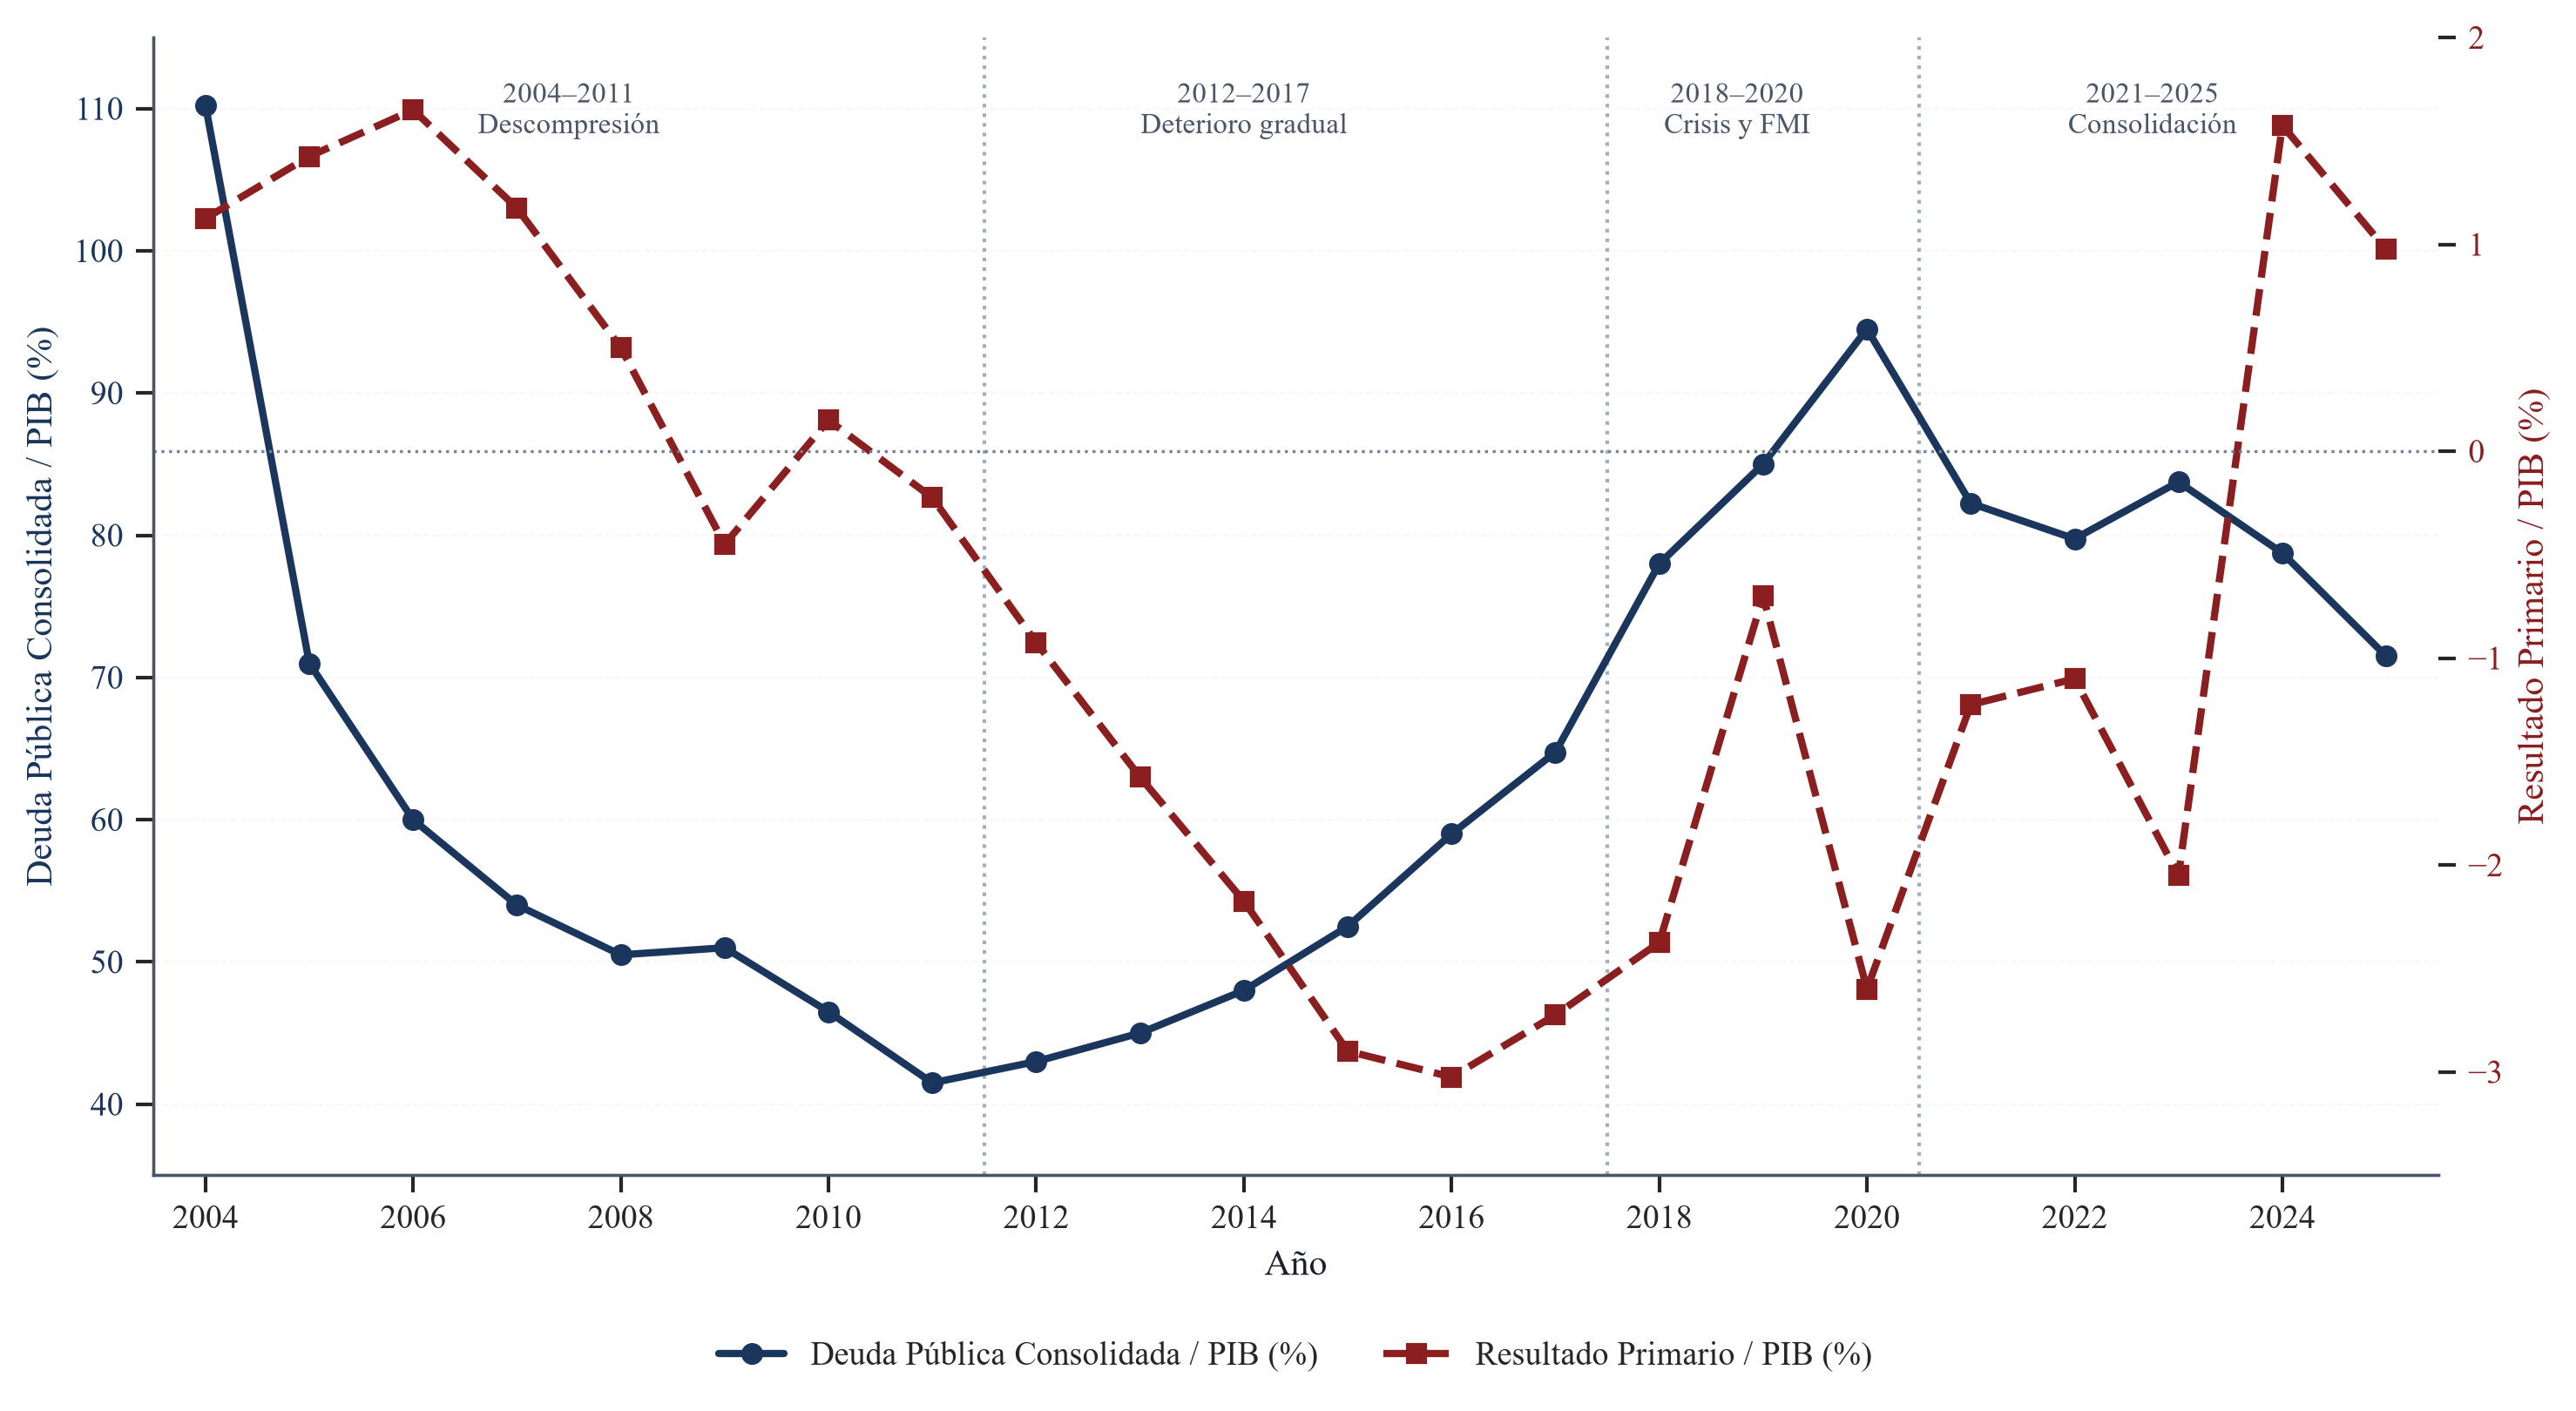
\includegraphics[width=0.88\textwidth]{figuras/fig5_1_deuda_resultado_primario.png}
\caption{Trayectoria Trimestral de la Deuda Pública sobre PIB y el Resultado Primario en Argentina (2004--2025).}
\label{fig:deuda_primario}
\end{figure}

---

\section{Modelos del Núcleo de la Tesis: Fundamentación Completa (APA 7)}

---

\subsection{Desagregación Temporal de Denton (1971) sin Indicador}

\subsubsection{1. ¿Para qué sirve?}
Permite transformar series anuales de baja frecuencia (en nuestro caso, el balance fiscal y el PIB de 1993 a 2003 del \textit{Compendio Fiscal de Hacienda}) en series trimestrales consistentes, de modo que la suma de los cuatro trimestres generados coincida de forma exacta e idéntica con el total anual auditado.

\subsubsection{2. ¿Por qué se utiliza frente a otras alternativas?}
Frente a la interpolación lineal simple o spline cúbico (que no garantizan la conservación del flujo anual acumulado), el algoritmo de Denton minimiza la suma de cuadrados de las diferencias entre períodos sucesivos. Además, frente al método de Chow-Lin o Denton proporcional con indicador, el método sin indicador se eligió porque no existía un indicador mensual homogéneo y continuo (el EMAE inicia en 2004). Emplear un indicador con quiebres metodológicos habría transferido errores de medición espurios a las series fiscales.

\subsubsection{3. ¿De dónde sale? (Referencia APA 7)}
\begin{mdframed}[style=apabox]
Denton, F. T. (1971). Adjustment of monthly or quarterly series to annual totals: An approach based on quadratic minimization. \textit{Journal of the American Statistical Association}, 66(333), 99--102. \url{https://doi.org/10.1080/01621459.1971.10482226}
\end{mdframed}

\subsubsection{4. Formulación Matemática Rigurosa}
Sea $y = [y_1, y_2, \dots, y_T]^\top$ el vector trimestral a estimar ($T=4M$) y $Y_A = [Y_1, \dots, Y_M]^\top$ el vector anual observado. El problema de optimización se formula como:

\begin{equation}
\min_{y} \, (D y)^\top (D y) \quad \text{sujeto a} \quad C y = Y_A
\end{equation}

Donde $D$ es la matriz de primeras diferencias de dimensión $(T-1) \times T$:
\begin{equation}
D = \begin{bmatrix}
-1 & 1 & 0 & \cdots & 0 & 0 \\
0 & -1 & 1 & \cdots & 0 & 0 \\
\vdots & \vdots & \ddots & \ddots & \vdots & \vdots \\
0 & 0 & 0 & \cdots & -1 & 1
\end{bmatrix}
\end{equation}

Y $C$ es la matriz de agregación temporal ($M \times T$):
\begin{equation}
C = \begin{bmatrix}
1 & 1 & 1 & 1 & 0 & 0 & 0 & 0 & \cdots & 0 \\
0 & 0 & 0 & 0 & 1 & 1 & 1 & 1 & \cdots & 0 \\
\vdots & \vdots & \vdots & \vdots & \vdots & \vdots & \vdots & \vdots & \ddots & \vdots \\
0 & 0 & 0 & 0 & 0 & 0 & 0 & 0 & \cdots & 1
\end{bmatrix}
\end{equation}

Planteando el Lagrangiano $\mathcal{L}(y, \lambda) = y^\top D^\top D y - 2 \lambda^\top (C y - Y_A)$, las condiciones de primer orden $\frac{\partial \mathcal{L}}{\partial y} = 2 D^\top D y - 2 C^\top \lambda = 0$ y $\frac{\partial \mathcal{L}}{\partial \lambda} = C y - Y_A = 0$ conducen a la solución analítica en forma cerrada:

\begin{equation}
y = (D^\top D)^{-1} C^\top \left[ C (D^\top D)^{-1} C^\top \right]^{-1} Y_A
\end{equation}

\subsubsection{5. Implementación en Código}
Se implementa en \texttt{codigo/ingesta\_datos/empalme\_historico\_pre2004.py} construyendo las matrices dispersas de diferencias y agregación y resolviendo el sistema lineal mediante \texttt{scipy.linalg.solve}.

\subsubsection{6. Aplicación a la Deuda Argentina}
Permitió extender la muestra hacia atrás hasta 1999T1 ($n=108$), incorporando el régimen de Convertibilidad y el default de 2001--2002 a pedido de la dirección de tesis, manteniendo la consistencia con las cuentas del Sector Público Nacional.

---

\subsection{Consolidación de Deuda con Pasivos del Banco Central}

\subsubsection{1. ¿Para qué sirve?}
Consolida el balance del Sector Público No Financiero (SPNF) con el balance cuasifiscal del Banco Central de la República Argentina (BCRA), computando la deuda pública total neta de tenencias intra-sector público.

\subsubsection{2. ¿Por qué se utiliza frente a otras alternativas?}
Analizar únicamente la deuda del SPNF subestima la vulnerabilidad del Estado, ya que en Argentina el déficit fiscal recurrente fue financiado mediante la colocación de pasivos monetarios remunerados del BCRA (LEBAC, LELIQ, NOTALIQ y Pases Pasivos), los cuales pagan tasas de interés de mercado y generan una carga cuasifiscal de vencimiento ultracorto.

\subsubsection{3. ¿De dónde sale? (Referencia APA 7)}
\begin{mdframed}[style=apabox]
Sargent, T. J., \& Wallace, N. (1981). Some unpleasant monetarist arithmetic. \textit{Federal Reserve Bank of Minneapolis Quarterly Review}, 5(3), 1--17.\\
Reinhart, C. M., \& Rogoff, K. S. (2011). The forgotten history of domestic debt. \textit{The Economic Journal}, 121(552), 319--350. \url{https://doi.org/10.1111/j.1468-0297.2011.02426.x}
\end{mdframed}

\subsubsection{4. Formulación Matemática}
La deuda pública consolidada neta sobre PIB ($d_t^{\text{cons}}$) se calcula como:

\begin{equation}
D_t^{\text{cons}} = D_t^{\text{SPNF}} + \text{Pasivos Remunerados BCRA}_t - \text{Títulos Públicos en Activo BCRA}_t
\end{equation}

\begin{equation}
d_t^{\text{cons}} = \frac{D_t^{\text{cons}}}{\text{PIB}_t}
\end{equation}

\begin{figure}[H]
\centering
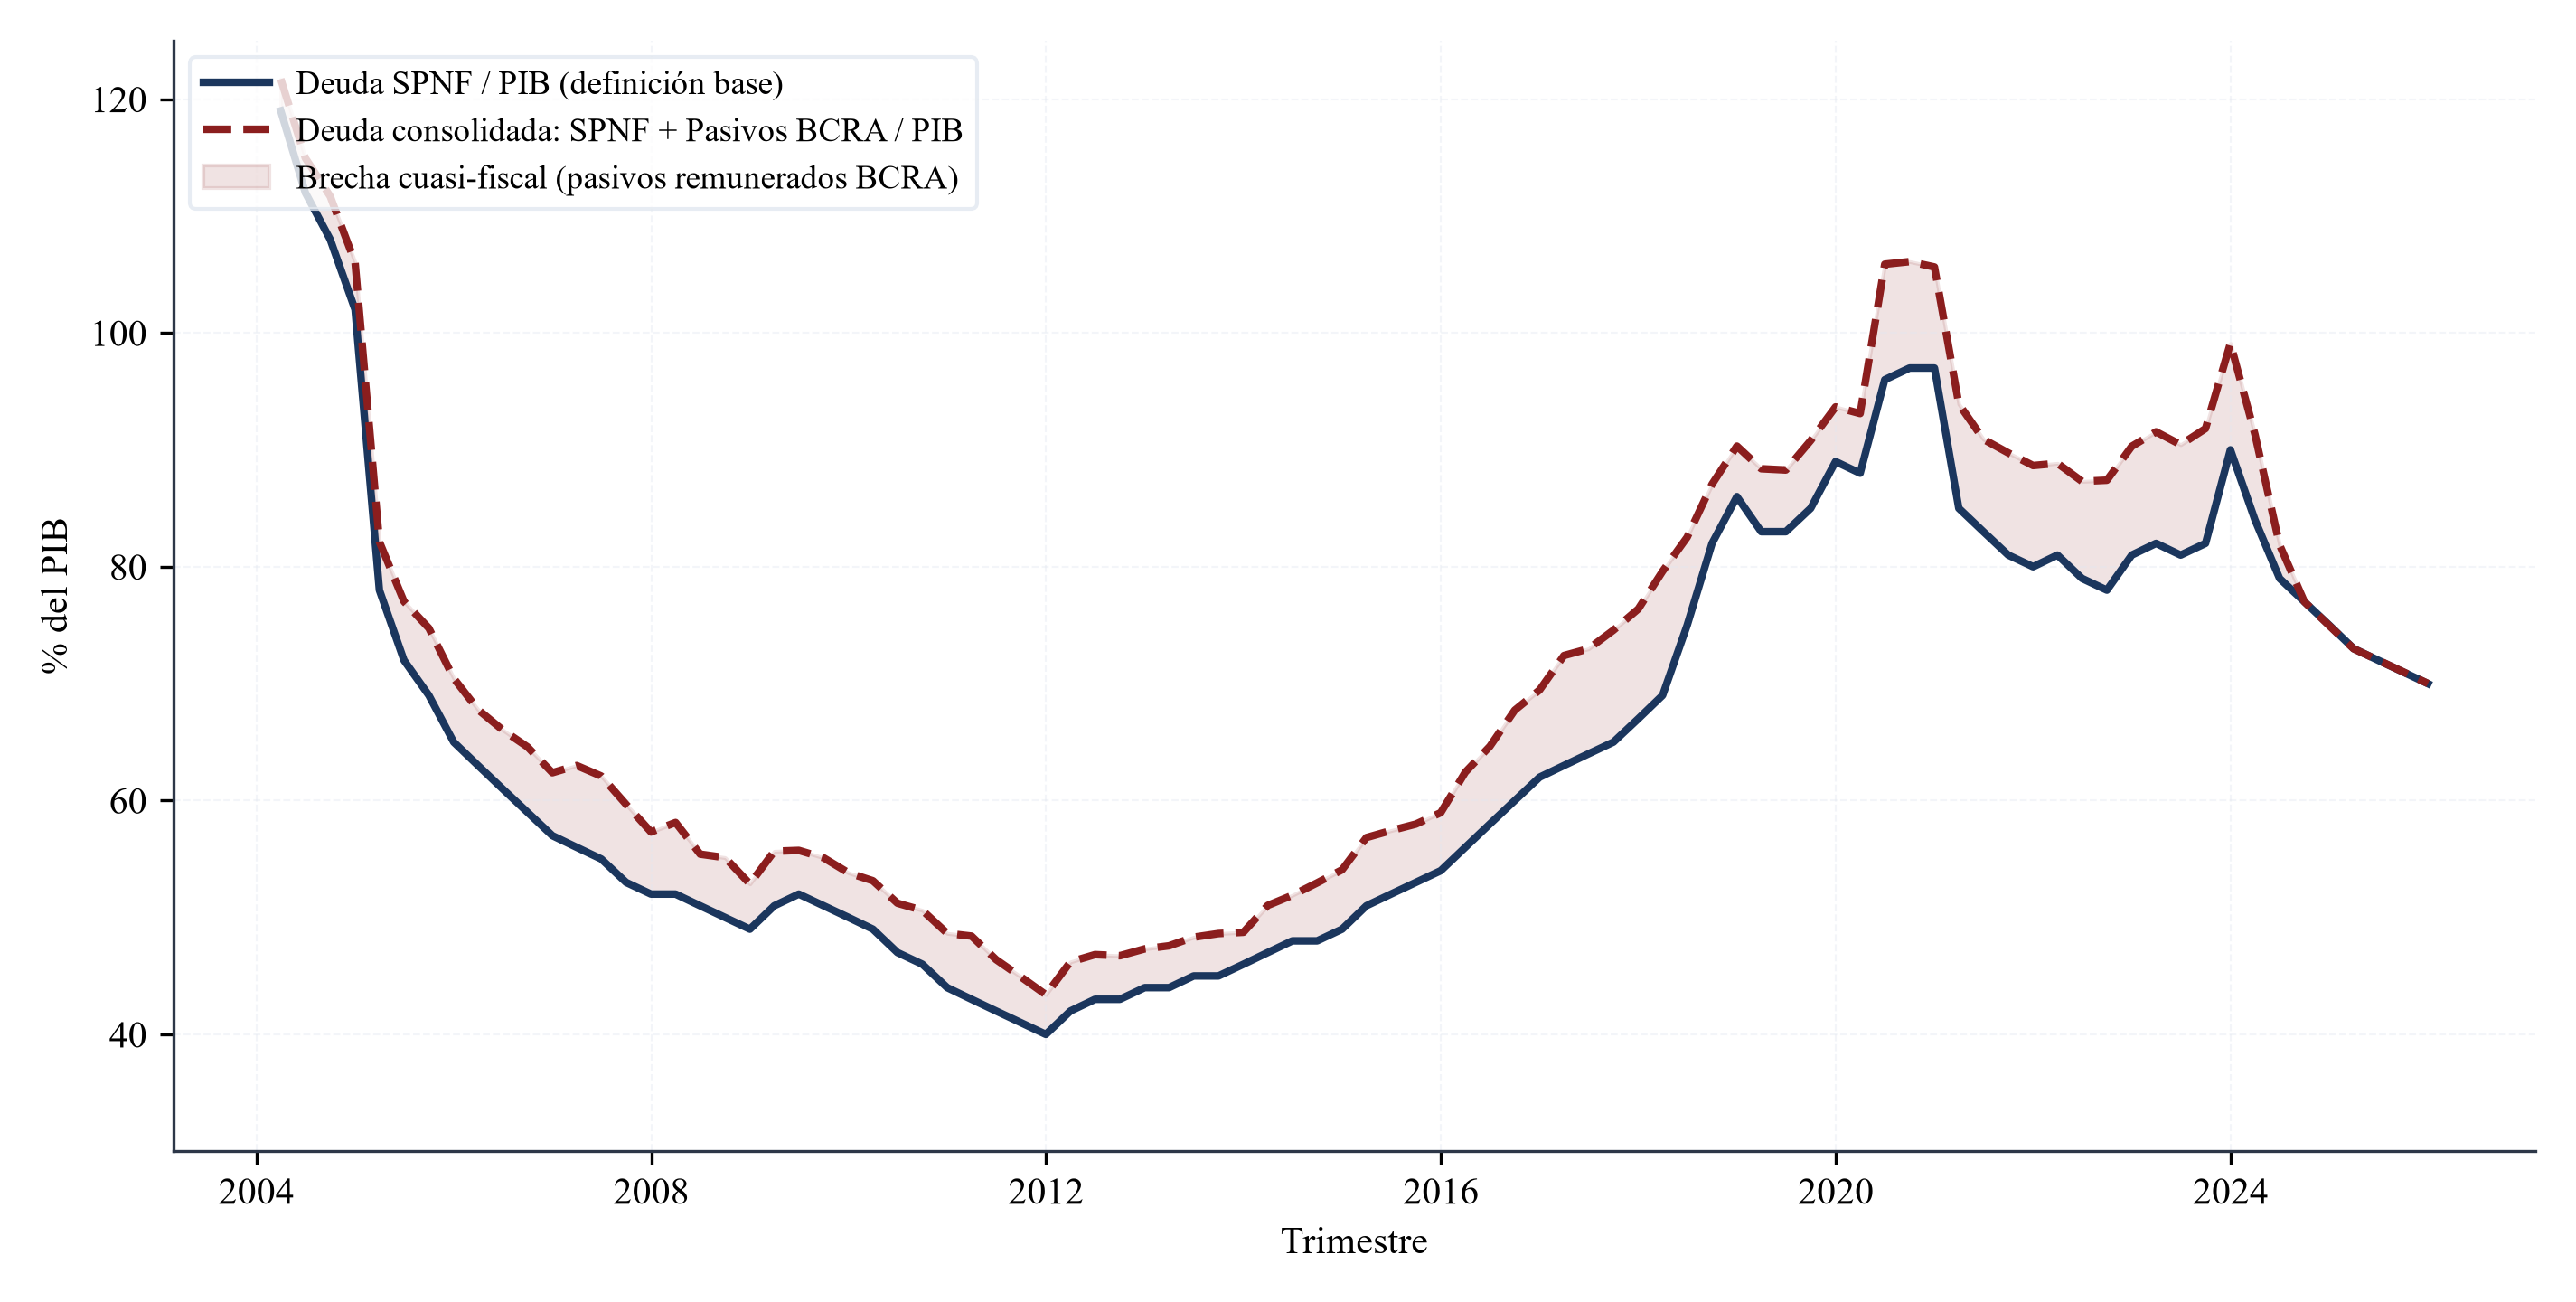
\includegraphics[width=0.85\textwidth]{figuras/figura_8_1_deuda_consolidada.png}
\caption{Comparación entre Deuda SPNF y Deuda Consolidada con Pasivos del BCRA (LELIQ/Pases).}
\label{fig:deuda_consolidada}
\end{figure}

---

\subsection{El Sistema VECM y Cointegración de Johansen (1991, 2000)}

\subsubsection{1. ¿Para qué sirve?}
Modela de manera conjunta y endógena la interacción dinámica entre el stock de deuda, el resultado primario, el riesgo soberano y el tipo de cambio real, permitiendo evaluar si el superávit primario reacciona como mecanismo de corrección de error hacia el equilibrio fiscal de largo plazo.

\subsubsection{2. ¿Por qué se utiliza frente a un VAR en diferencias?}
Por el **Teorema de Representación de Granger (Engle \& Granger, 1987)**: si las series son no estacionarias $I(1)$ y están cointegradas, un VAR en primeras diferencias ignora el atractor de equilibrio $\alpha \beta^\top Y_{t-1}$, incurriendo en un sesgo grave de especificación dinámica. El VECM es la única estructura que combina dinámicas transitorias con cointegración estructural.

\subsubsection{3. ¿De dónde sale? (Referencia APA 7)}
\begin{mdframed}[style=apabox]
Johansen, S. (1991). Estimation and hypothesis testing of cointegration vectors in Gaussian vector autoregressive models. \textit{Econometrica}, 59(6), 1551--1580. \url{https://doi.org/10.2307/2938278}\\
Johansen, S., Mosconi, R., \& Nielsen, B. (2000). Cointegration analysis in the presence of structural breaks in the deterministic trend. \textit{The Econometrics Journal}, 3(2), 216--249. \url{https://doi.org/10.1111/1368-423X.00047}
\end{mdframed}

\subsubsection{4. Formulación Matemática Rigurosa}
Sea $Y_t = [d_t, pb_t, \text{EMBI}_t, \text{TCRM}_t]^\top \sim I(1)$ y $\tilde{y}_t \sim I(0)$ la brecha del producto. El modelo VECM de orden $p$ se define como:

\begin{equation}
\Delta Y_t = \mu + \Pi Y_{t-1} + \sum_{i=1}^{p-1} \Gamma_i \Delta Y_{t-i} + \Phi \tilde{y}_t + \varepsilon_t
\end{equation}

Donde $\Pi = \alpha \beta^\top$, siendo $\alpha$ la matriz de velocidades de ajuste ($4 \times r$) y $\beta$ la matriz de vectores de cointegración ($4 \times r$).
El procedimiento de máxima verosimilitud de Johansen resuelve:

\begin{equation}
|\lambda S_{11} - S_{10} S_{00}^{-1} S_{01}| = 0
\end{equation}

Y calcula los estadísticos de contraste:
\begin{equation}
\lambda_{\text{trace}}(r) = -T \sum_{i=r+1}^{K} \ln(1 - \hat{\lambda}_i), \quad \lambda_{\max}(r, r+1) = -T \ln(1 - \hat{\lambda}_{r+1})
\end{equation}

\subsubsection{5. Aplicación y Resultados en la Tesis}
En la muestra homogénea 2004--2025 ($n=87$), Johansen rechaza $r=0$ y selecciona $r=1$ de forma unánime ($p < 0.05$). La velocidad de ajuste del superávit primario hacia el equilibrio de Bohn es:
\begin{equation}
\alpha_{pb} = 0.0014 \quad (p = 0.559) \quad \text{en ventana homogénea}
\end{equation}
\begin{equation}
\alpha_{pb} = 0.0044 \quad (p = 0.204) \quad \text{en ventana ampliada ($n=108$)}
\end{equation}
En ambos casos, $\alpha_{pb}$ es estadísticamente igual a cero, confirmando la inoperancia de una regla fiscal activa.

---

\subsection{Estimador DOLS e IV-2SLS (Stock \& Watson, 1993; Caner \& Hansen, 2004)}

\subsubsection{1. ¿Para qué sirve?}
Proporciona una estimación superconsistente de la ecuación de reacción fiscal de Bohn en un marco de ecuación única, corrigiendo la correlación de segundo orden y tratando la endogeneidad contemporánea del riesgo soberano mediante variables instrumentales.

\subsubsection{2. ¿Por qué se utiliza frente al OLS estático?}
El estimador OLS estático en regresiones de cointegración sufre de sesgo de muestra finita debido a la correlación asintótica entre las innovaciones de la ecuación y los regresores integrados. DOLS elimina este sesgo mediante la inclusión de adelantos y rezagos de las primeras diferencias ($\Delta d_{t-j}$).

\subsubsection{3. ¿De dónde sale? (Referencia APA 7)}
\begin{mdframed}[style=apabox]
Stock, J. H., \& Watson, M. W. (1993). A simple estimator of cointegrating vectors in higher order integrated systems. \textit{Econometrica}, 61(4), 783--820. \url{https://doi.org/10.2307/2951763}\\
Staiger, D., \& Stock, J. H. (1997). Instrumental variables regression with weak instruments. \textit{Econometrica}, 65(3), 557--586. \url{https://doi.org/10.2307/2171753}
\end{mdframed}

\subsubsection{4. Formulación Matemática}
La ecuación DOLS con $m=4$ adelantos y rezagos se formula como:

\begin{equation}
pb_t = \beta_0 + \rho d_{t-1} + \gamma \tilde{y}_t + \delta \text{EMBI}_t + \theta \text{TCRM}_t + \sum_{j=-m}^{m} \psi_j \Delta d_{t-j} + \varepsilon_t
\end{equation}

Para el IV-2SLS, se instrumenta $\text{EMBI}_t$ mediante $Z_t = [\text{VIX}_t, \text{EMB\_Spread}_t]$:
\begin{itemize}
    \item **Primera Etapa**: $\text{EMBI}_t = Z_t \Pi + X_t \Gamma + v_t \implies F_{1ra} = 13.00 > 10$.
    \item **Test de Wu-Hausman**: $F = 7.32 \quad (p = 0.009) \implies$ Se rechaza la exogeneidad del EMBI+.
    \item **Test de Sargan**: $J = 0.608 \quad (p = 0.436) \implies$ Instrumentos válidos.
\end{itemize}

\begin{figure}[H]
\centering
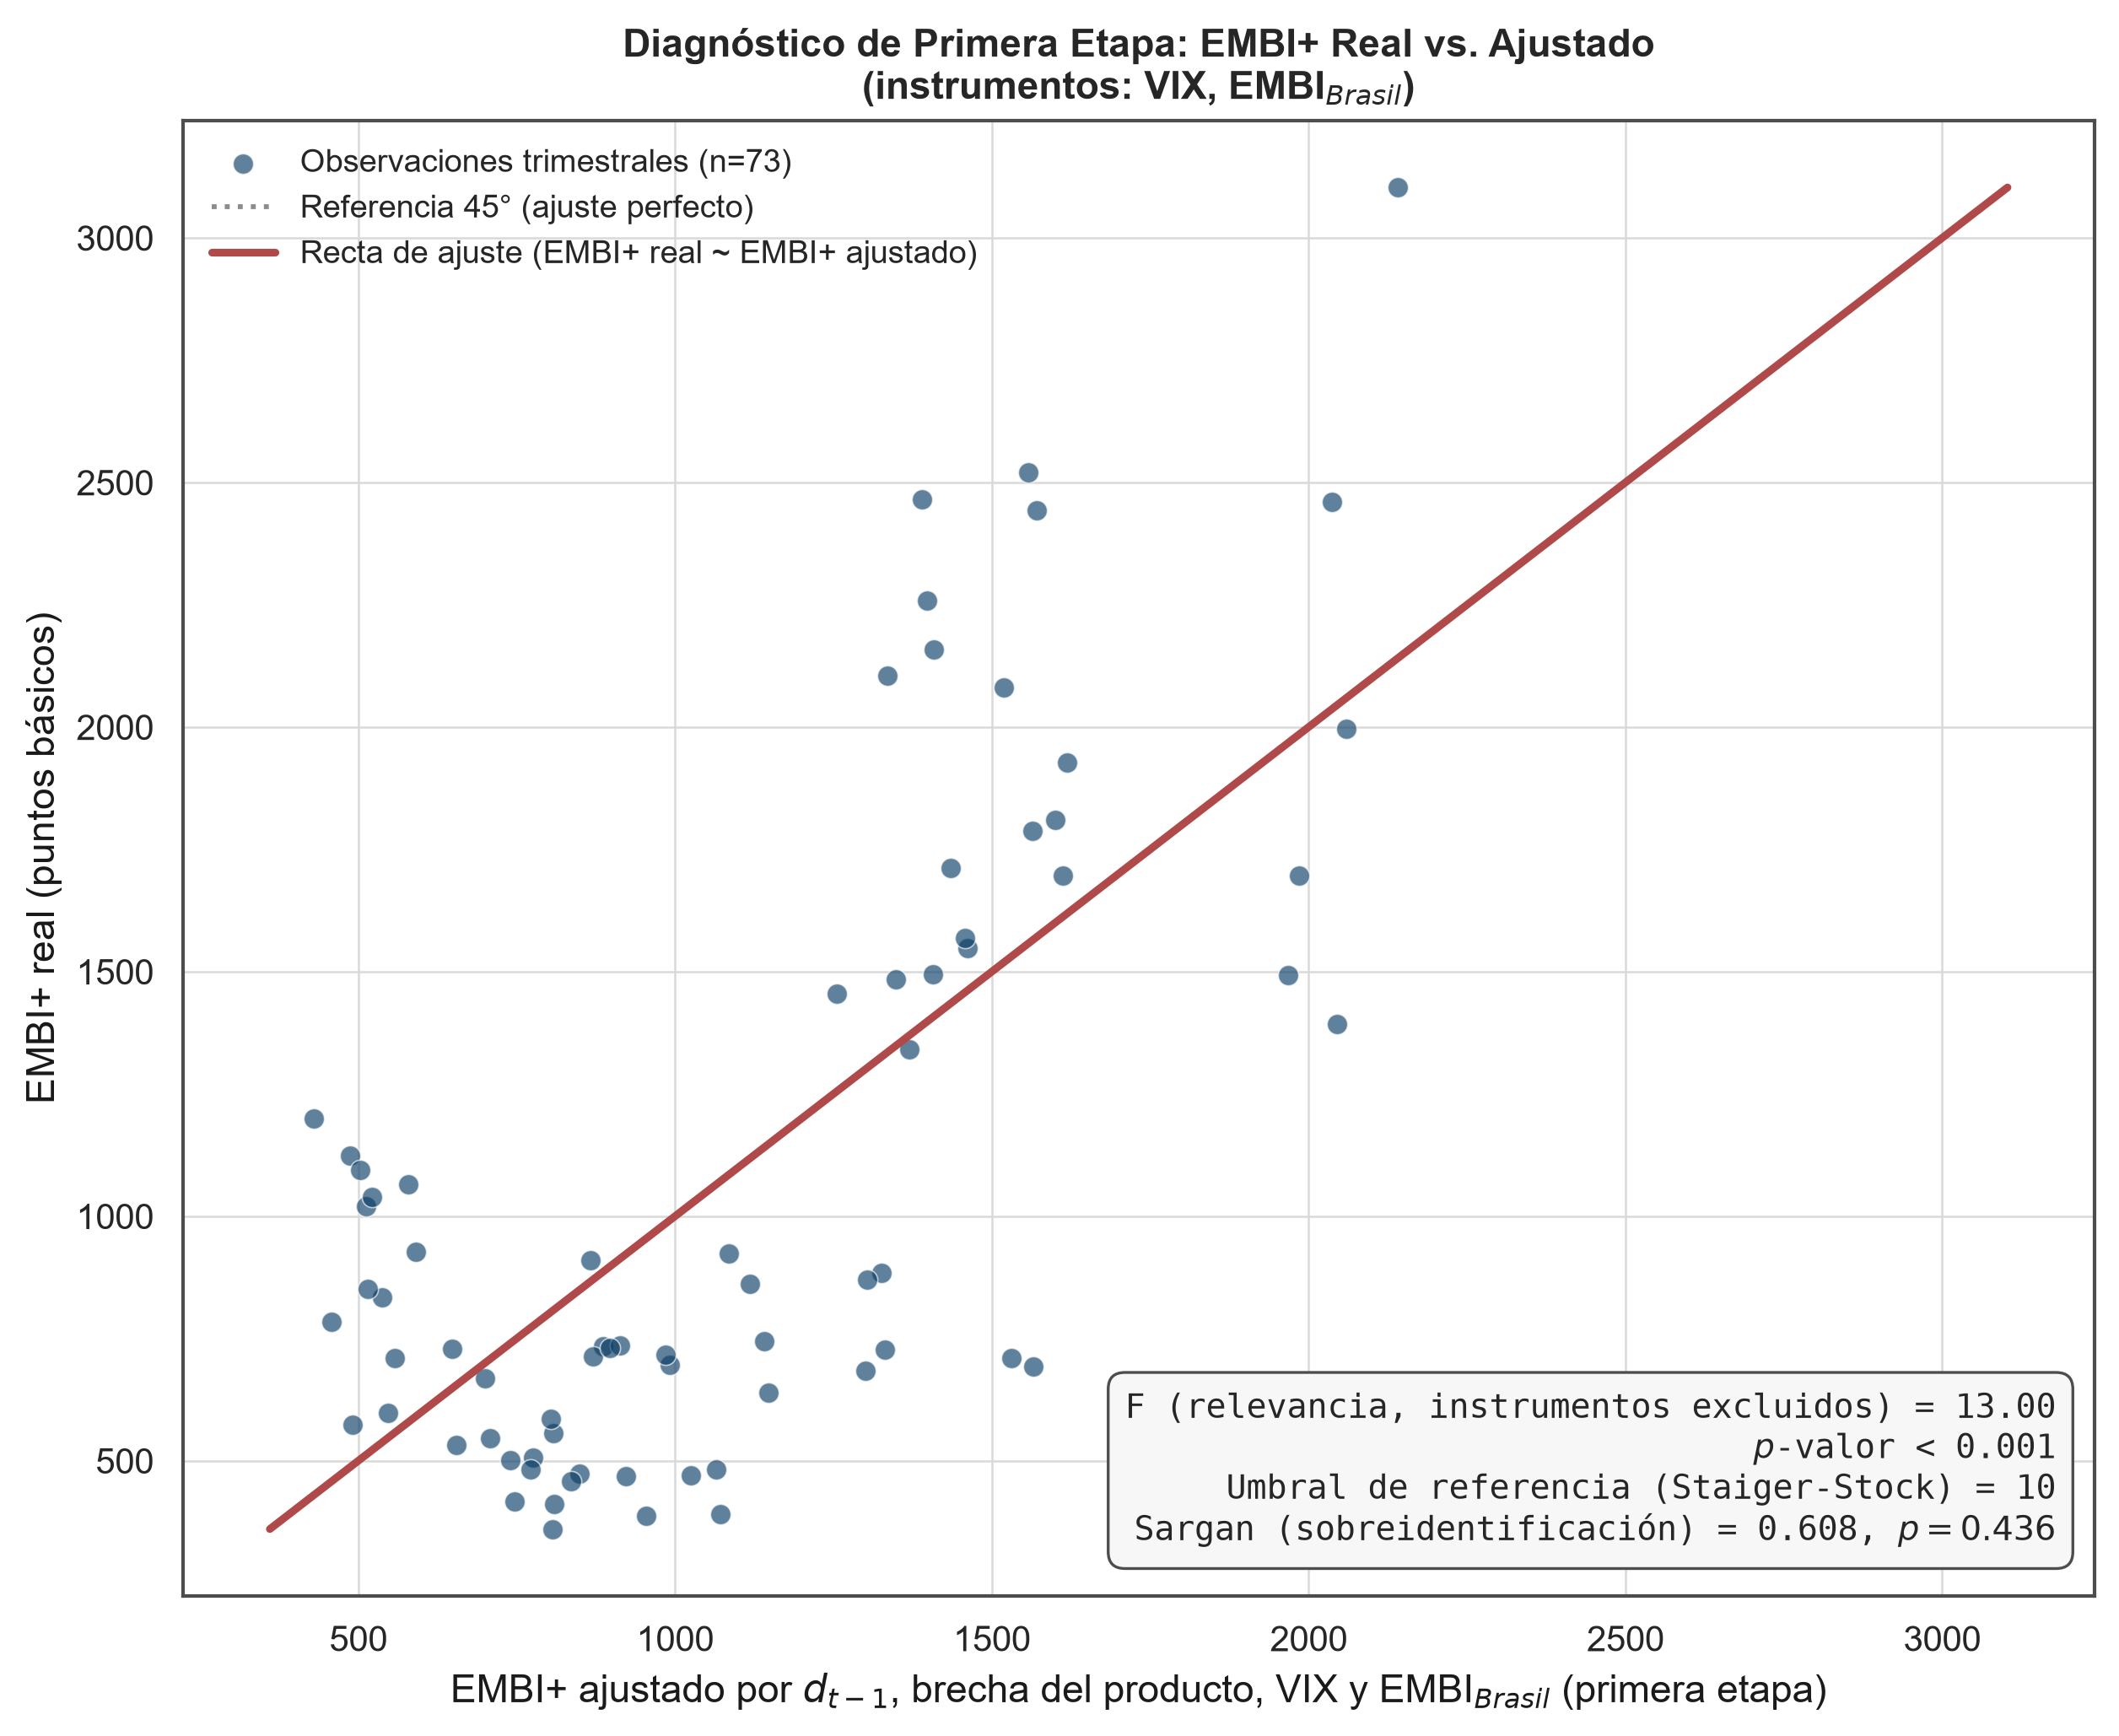
\includegraphics[width=0.82\textwidth]{figuras/fig6_1_diagnostico_primera_etapa.png}
\caption{Diagnóstico de Primera Etapa IV-2SLS: Relevancia y Ortogonalidad de Instrumentos.}
\label{fig:iv_2sls}
\end{figure}

---

\subsection{Quiebres Estructurales Múltiples de Bai y Perron (2003)}

\subsubsection{1. ¿Para qué sirve?}
Identifica de manera puramente endógena las fechas exactas de ruptura estructural en la trayectoria de la deuda pública argentina, sin imponer quiebres basados en eventos históricos arbitrarios.

\subsubsection{2. ¿Por qué se utiliza frente al test de Chow o Zivot-Andrews?}
El test de Chow requiere conocer la fecha de quiebre a priori. El test de Zivot-Andrews permite un único quiebre endógeno. El algoritmo de Bai y Perron permite $m$ quiebres múltiples simultáneos, evaluando todas las posibles particiones mediante programación dinámica exacta.

\subsubsection{3. ¿De dónde sale? (Referencia APA 7)}
\begin{mdframed}[style=apabox]
Bai, J., \& Perron, P. (2003). Computation and analysis of multiple structural change models. \textit{Journal of Applied Econometrics}, 18(1), 1--22. \url{https://doi.org/10.1002/jae.659}
\end{mdframed}

\subsubsection{4. Formulación Matemática}
Para un modelo con $m$ quiebres ($m+1$ regímenes):

\begin{equation}
y_t = x_t^\top \beta + z_t^\top \delta_j + u_t \quad (t = T_{j-1}+1, \dots, T_j; \, j=1, \dots, m+1)
\end{equation}

El algoritmo resuelve por programación dinámica de Bellman:
\begin{equation}
\text{SSR}(T_1, \dots, T_m) = \sum_{j=1}^{m+1} \sum_{t=T_{j-1}+1}^{T_j} \left( y_t - z_t^\top \hat{\delta}_j \right)^2
\end{equation}
Seleccionando el número óptimo de quiebres mediante el criterio BIC de Yao (1988):
\begin{equation}
\text{BIC}(m) = \ln\left( \frac{\text{SSR}(m)}{T} \right) + m \cdot \frac{K \ln(T)}{T}
\end{equation}

\begin{figure}[H]
\centering
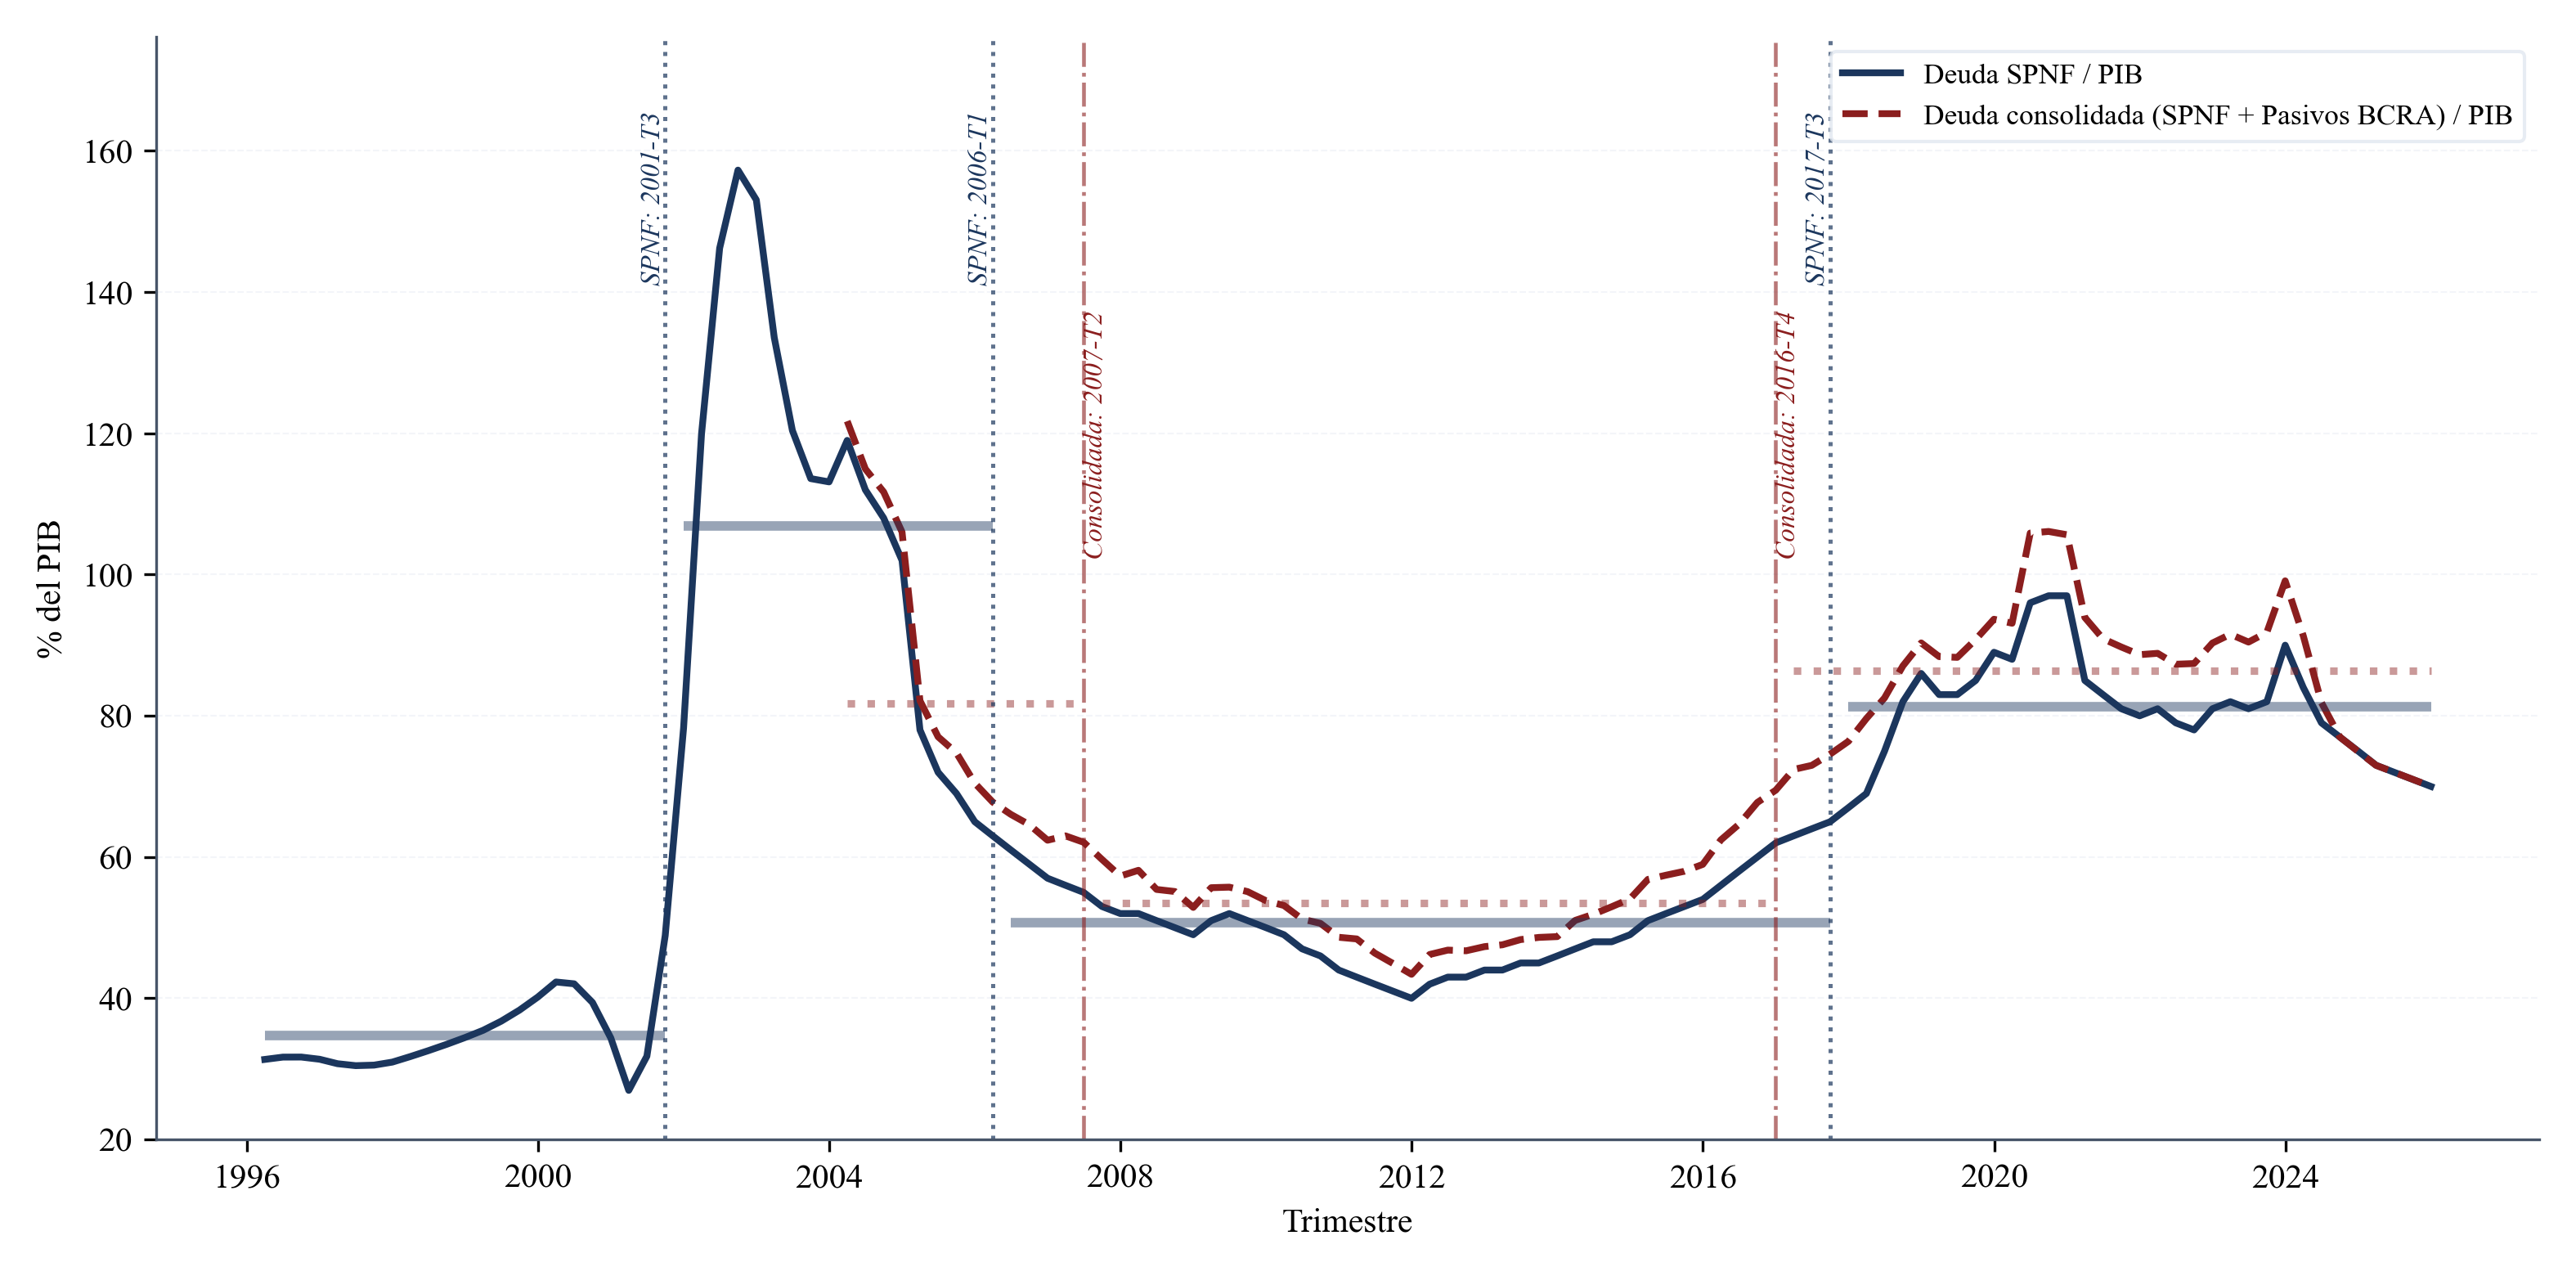
\includegraphics[width=0.82\textwidth]{figuras/figura_9_1_bai_perron.png}
\caption{Cronología y Estimación de Quiebres Estructurales Múltiples (Bai y Perron).}
\label{fig:bai_perron}
\end{figure}

---

\subsection{Modelo de Umbral No Lineal de Hansen (1999, 2000)}

\subsubsection{1. ¿Para qué sirve?}
Permite contrastar formalmente la hipótesis de **fatiga fiscal** (Ghosh et al., 2013), evaluando si la capacidad o disposición del gobierno para generar superávit primario colapsa a partir de un nivel crítico de estrés financiero.

\subsubsection{2. ¿Por qué se utiliza frente a una regresión cuadrática/cúbica tradicional?}
Las funciones polinómicas imponen una forma funcional suave y simétrica que no refleja la naturaleza discontinua de las crisis de deuda. El modelo de Hansen identifica el punto de quiebre endógeno ($\tau^*$) y calcula su significatividad mediante remuestreo estocástico Sup-LM, sorteando el problema del parámetro no identificado bajo la hipótesis nula (Davies, 1987).

\subsubsection{3. ¿De dónde sale? (Referencia APA 7)}
\begin{mdframed}[style=apabox]
Hansen, B. E. (2000). Sample splitting and threshold estimation. \textit{Econometrica}, 68(3), 575--603. \url{https://doi.org/10.1111/1468-0262.00124}\\
Ghosh, A. R., Kim, J. I., Mendoza, E. G., Ostry, J. D., \& Qureshi, M. S. (2013). Fiscal fatigue, fiscal space and debt sustainability in advanced economies. \textit{The Economic Journal}, 123(566), F4--F30. \url{https://doi.org/10.1111/ecoj.12010}
\end{mdframed}

\subsubsection{4. Formulación Matemática}
Sobre la primera diferencia estacionaria $\Delta pb_t$:

\begin{equation}
\Delta pb_t = \beta_1 d_{t-1} \cdot \mathbb{I}(\text{EMBI}_{t-1} \le \gamma) + \beta_2 d_{t-1} \cdot \mathbb{I}(\text{EMBI}_{t-1} > \gamma) + \gamma^\top X_t + \varepsilon_t
\end{equation}

Con el estimador de mínimos cuadrados concentrados:
\begin{equation}
\hat{\gamma} = \arg\min_{\gamma \in \Gamma} S_n(\gamma), \quad F_n = \sup_{\gamma \in \Gamma} F_n(\gamma)
\end{equation}
El valor $p$ se computa por remuestreo no paramétrico ($B = 1.000$ réplicas), obteniendo $\tau^* = 2083$ pb ($p < 0.001$) con $\beta_1 = 0.0184$ ($p=0.001$) y $\beta_2 = 0.0077$ ($p=0.030$).

\begin{figure}[H]
\centering
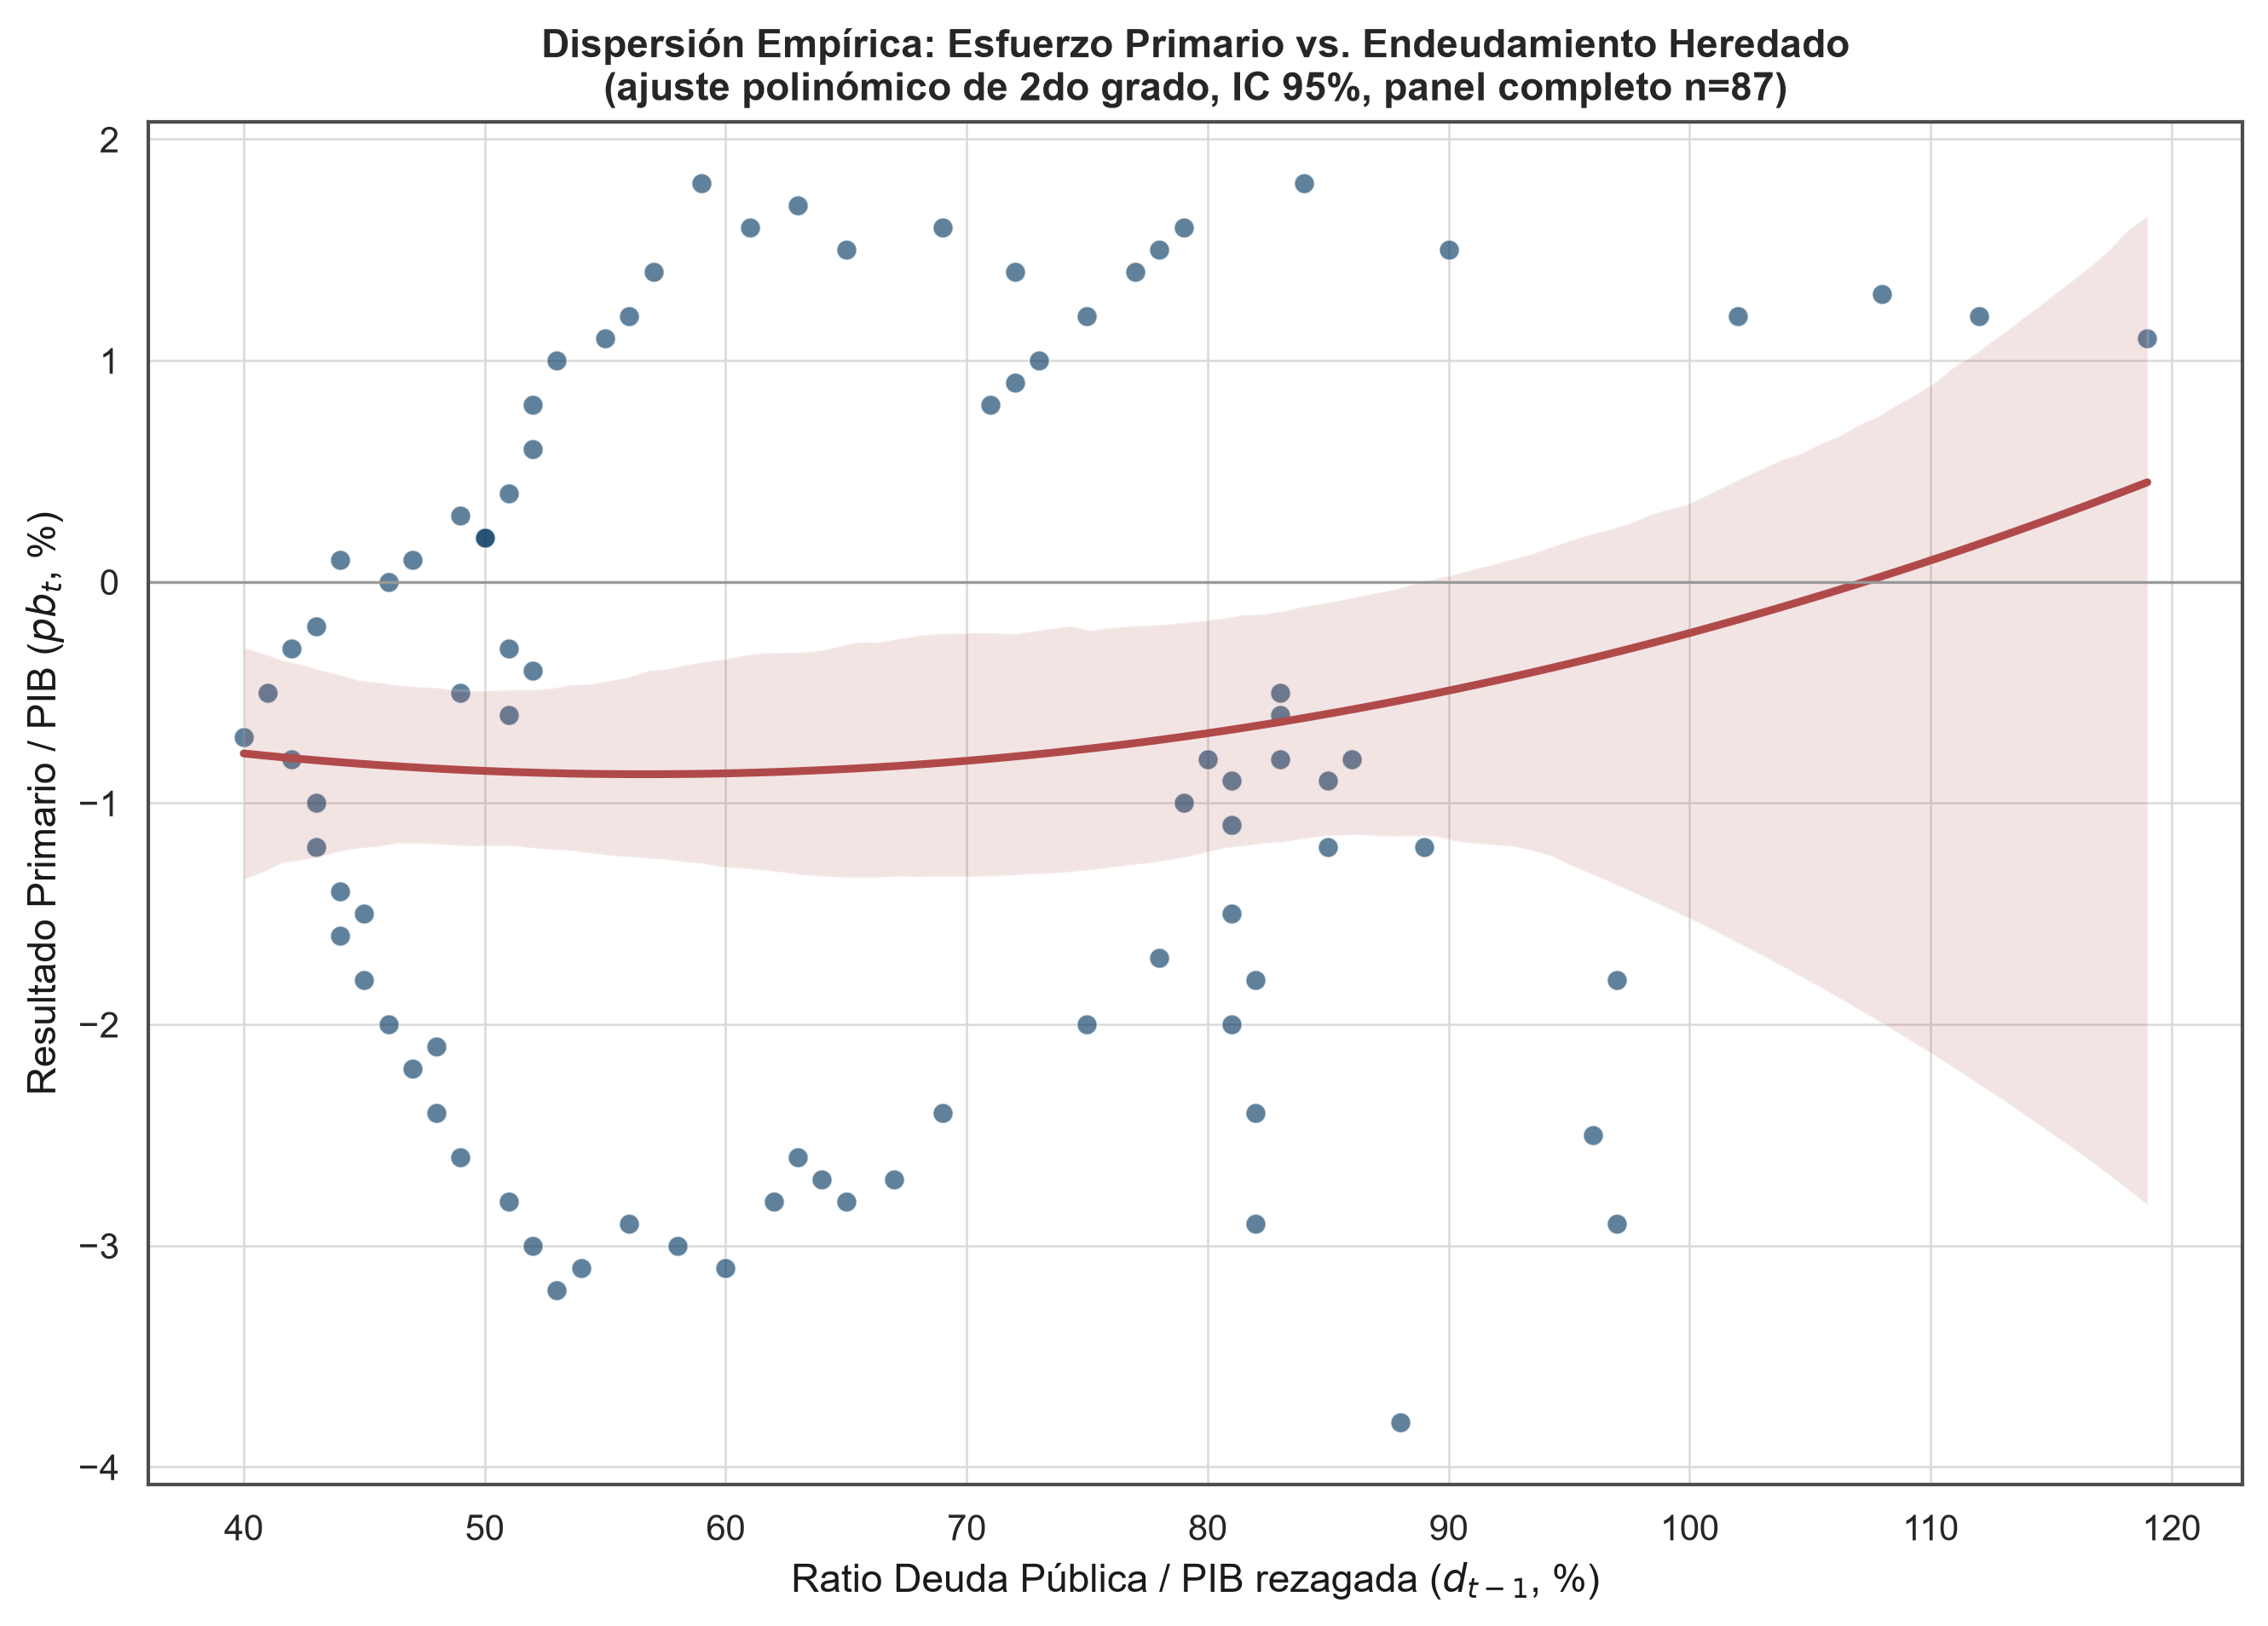
\includegraphics[width=0.82\textwidth]{figuras/fig5_3_dispersion_fatiga_fiscal.png}
\caption{Diagrama de Dispersión y Ajuste No Lineal de Fatiga Fiscal.}
\label{fig:fatiga_fiscal}
\end{figure}

---

\subsection{Análisis de Sostenibilidad de Deuda (DSA) Estocástico con DCC-GARCH}

\subsubsection{1. ¿Para qué sirve?}
Proyecta la trayectoria estocástica del ratio Deuda/PIB hacia 2035 mediante 1.000 simulaciones de Monte Carlo, calculando la probabilidad de insolvencia bajo colas pesadas e interdependencia macroeconómica dinámica.

\subsubsection{2. ¿Por qué se utiliza frente a escenarios deterministas estáticos?}
Los ejercicios deterministas tradicionales del FMI evalúan shocks aislados e ignoran las correlaciones cruzadas no lineales y el riesgo de cola pesada. La combinación de una cópula $t$-Student con correlaciones dinámicas DCC-GARCH captura la concentración de volatilidad y la ocurrencia simultánea de shocks extremos (devaluación, corte de crédito y recesión).

\subsubsection{3. ¿De dónde sale? (Referencia APA 7)}
\begin{mdframed}[style=apabox]
Celasun, O., Debrun, X., \& Ostry, J. D. (2006). Primary surplus behavior and risks to fiscal sustainability in emerging market countries: A ``fan-chart'' approach. \textit{IMF Staff Papers}, 53(3), 401--425. \url{https://doi.org/10.5089/9781451864199.001}\\
Engle, R. (2002). Dynamic conditional correlation: A simple class of multivariate generalized autoregressive conditional heteroskedasticity models. \textit{Journal of Business \& Economic Statistics}, 20(3), 339--350. \url{https://doi.org/10.1198/073500102288618487}
\end{mdframed}

\subsubsection{4. Formulación Matemática}
La ley de movimiento no lineal de la deuda es:

\begin{equation}
d_t = d_{t-1} \left( \frac{1 + r_t}{1 + g_t} \right) - pb_t + sft_t
\end{equation}

Donde la tasa de interés real ponderada es:
\begin{equation}
r_t = \alpha_d r_{d,t} + (1 - \alpha_d) \left[ (1 + r_{f,t})(1 + \Delta tc_t) - 1 \right]
\end{equation}

Las perturbaciones siguen $\varepsilon_t \sim t_\nu(0, H_t)$ con $\nu = 4.8$ grados de libertad, donde la matriz condicional de covarianza dinámica se descompone según Engle (2002):
\begin{equation}
H_t = D_t R_t D_t, \quad R_t = \text{diag}(Q_t)^{-1/2} Q_t \text{diag}(Q_t)^{-1/2}
\end{equation}
\begin{equation}
Q_t = (1 - a - b)\bar{Q} + a (\epsilon_{t-1} \epsilon_{t-1}^\top) + b Q_{t-1}
\end{equation}

\begin{figure}[H]
\centering
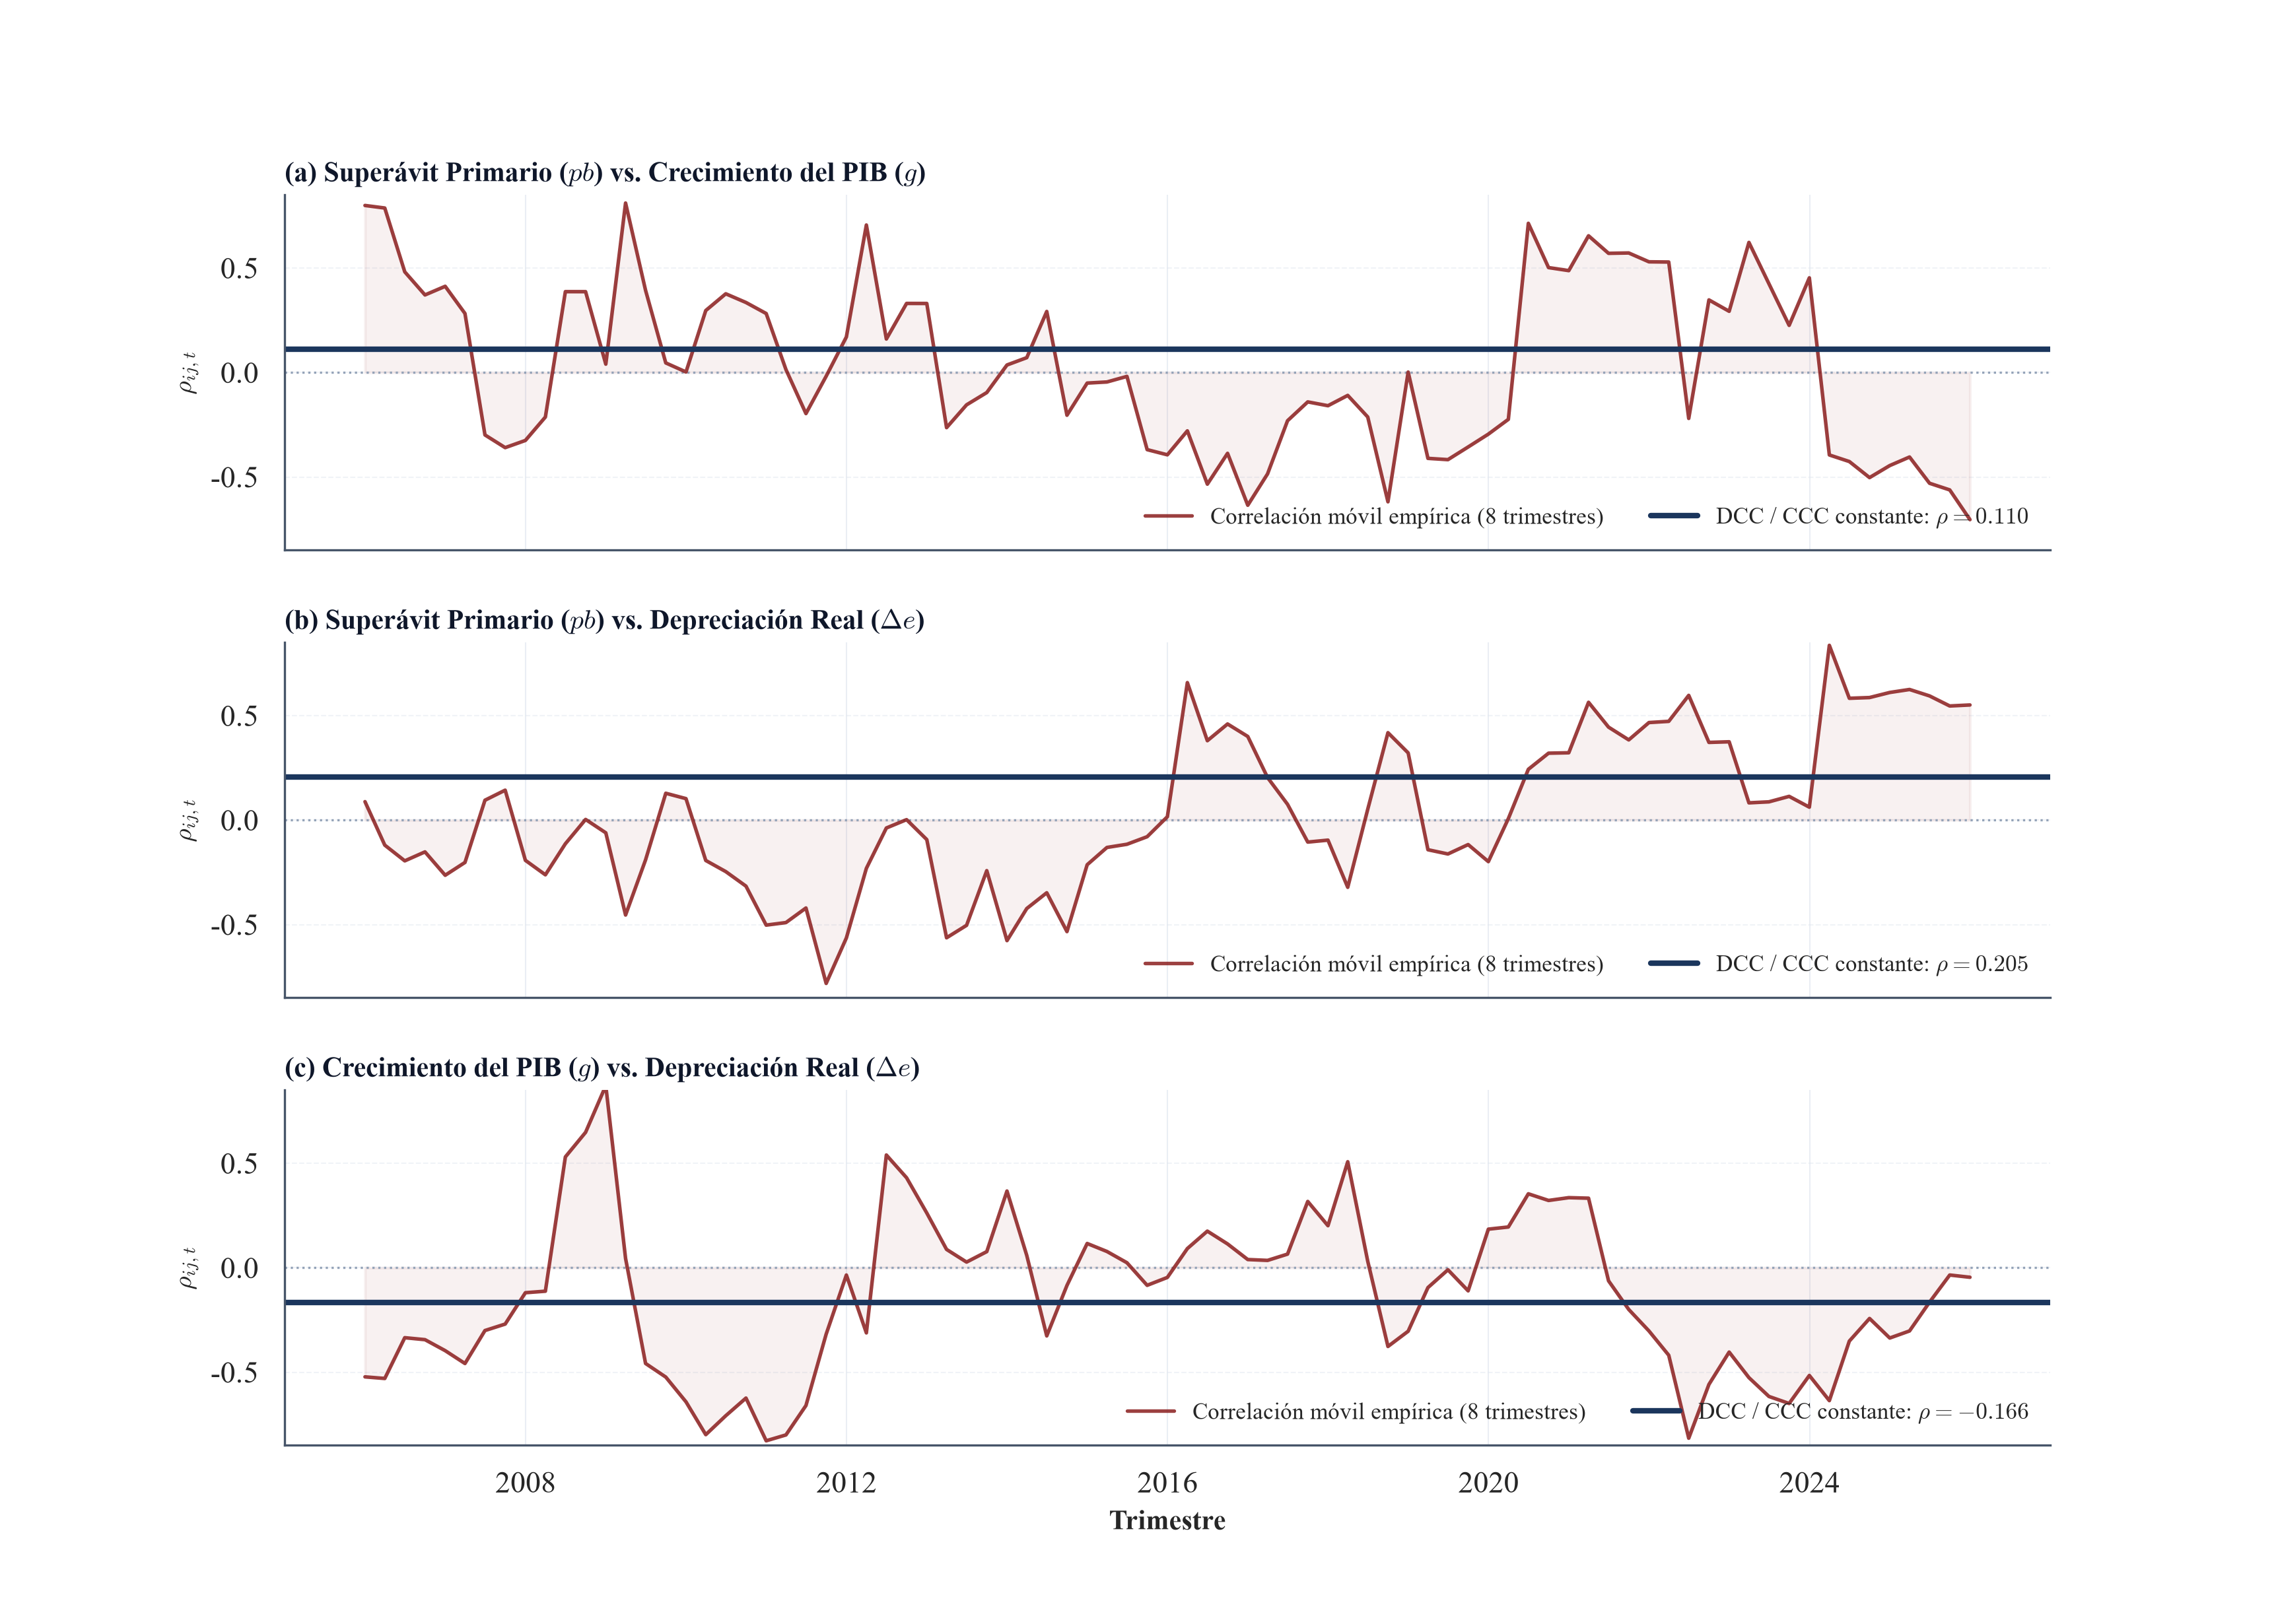
\includegraphics[width=0.80\textwidth]{figuras/figura_10_1_dcc_correlacion_dinamica.png}
\caption{Evolución Temporal de las Correlaciones Dinámicas Condicionales (DCC-GARCH).}
\label{fig:dcc_garch}
\end{figure}

\begin{figure}[H]
\centering
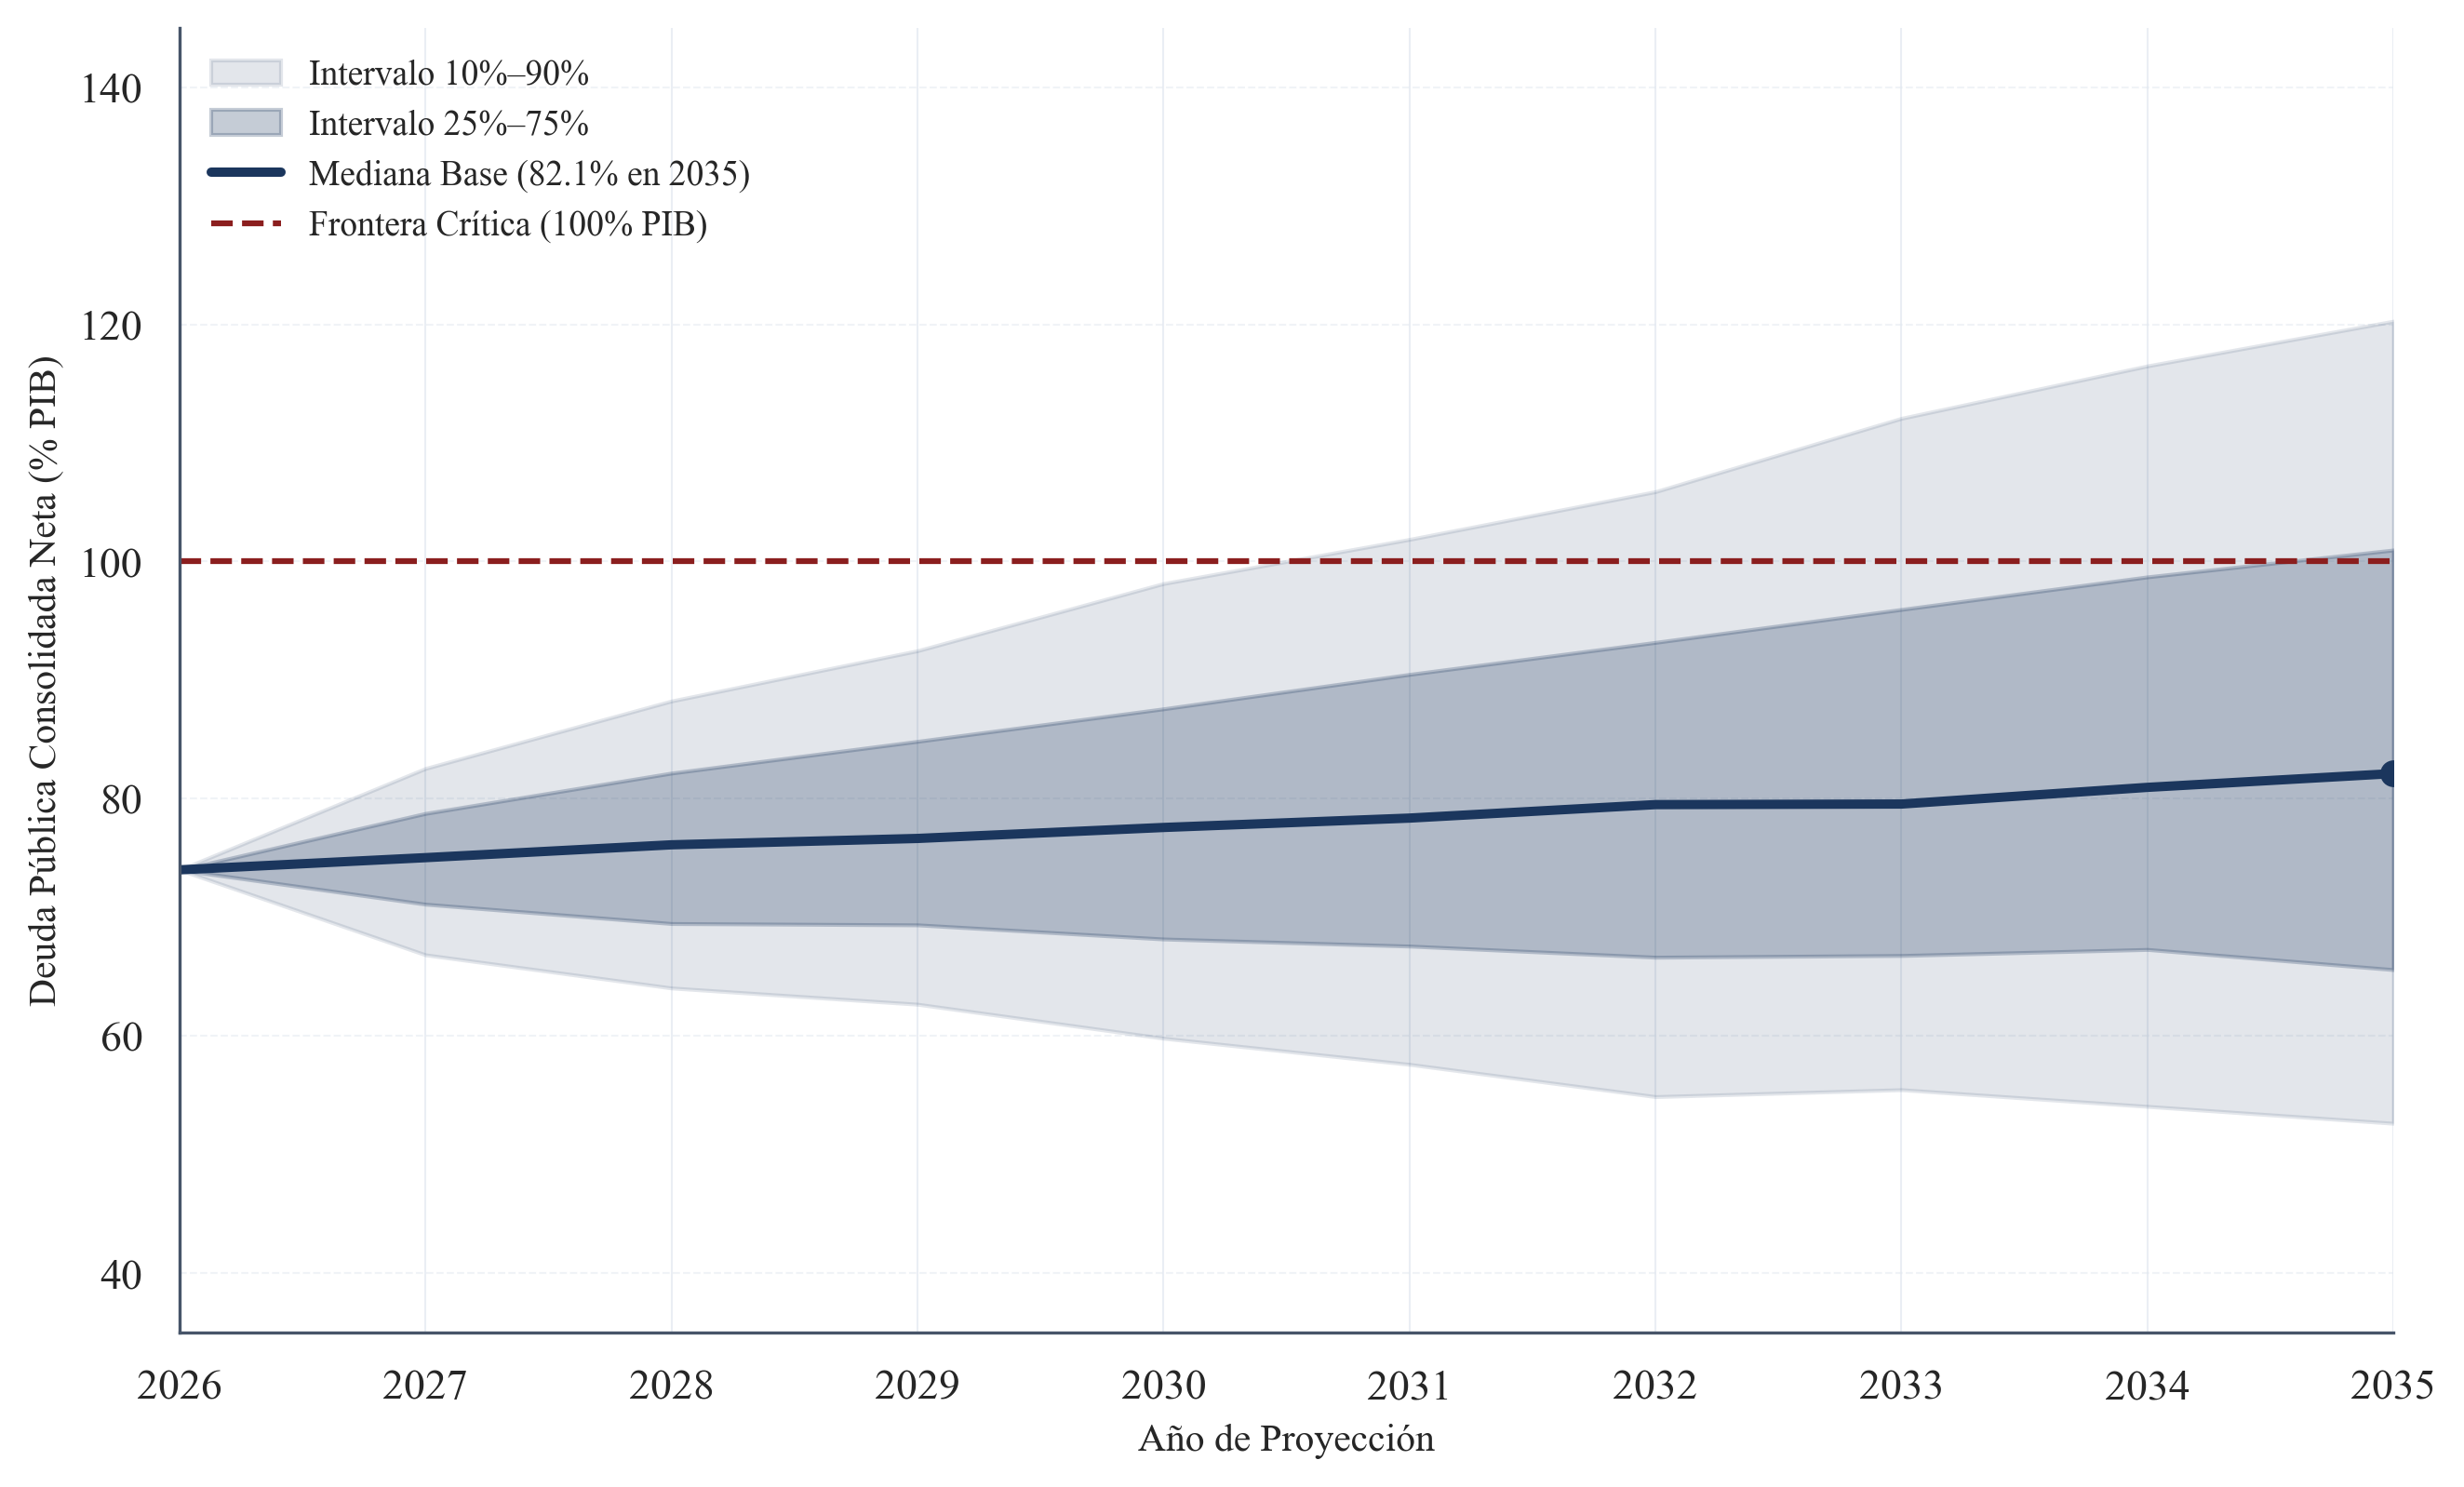
\includegraphics[width=0.85\textwidth]{figuras/dsa_grafico_abanico.png}
\caption{Proyecciones Estocásticas de Sostenibilidad hacia 2035 (Gráfico en Abanico).}
\label{fig:dsa_abanico}
\end{figure}

---

\section{Propuestas Cuantitativas de Frontera para el Jurado}

---

\subsection{Threshold VECM (TVECM) Multivariado de Hansen y Seo (2002)}

\subsubsection{1. ¿Para qué sirve?}
Permite unificar la estimación multivariada del VECM y la teoría de umbrales no lineales en un único sistema matricial, evaluando si el vector de velocidades de ajuste ($\alpha$) y la relación de cointegración conmuta de régimen entre períodos normales y períodos de estrés de riesgo soberano.

\subsubsection{2. ¿Por qué se utiliza frente a un VECM lineal tradicional?}
Un VECM lineal tradicional asume que la velocidad de corrección hacia el equilibrio fiscal de largo plazo es constante e idéntica tanto si el riesgo país es de 400 puntos básicos como si es de 2.500 puntos básicos. El TVECM permite que la dinámica de ajuste sea discontinua y dependa del estado del mercado de crédito internacional.

\subsubsection{3. ¿De dónde sale? (Referencia APA 7)}
\begin{mdframed}[style=apabox]
Hansen, B. E., \& Seo, B. (2002). Testing for two-regime threshold cointegration in vector error-correction models. \textit{Journal of Econometrics}, 110(2), 293--318. \url{https://doi.org/10.1016/S0304-4076(01)00097-4}
\end{mdframed}

\subsubsection{4. Formulación Matemática Rigurosa}
Sea $Y_t = [d_t, pb_t, \text{EMBI}_t, \text{TCRM}_t]^\top$. El modelo TVECM de dos regímenes con variable de umbral $w_{t-1} = \text{EMBI}_{t-1}$ y vector de cointegración $\beta$ se expresa como:

\begin{equation}
\Delta Y_t = \begin{cases}
\mu_1 + \alpha_1 \beta^\top Y_{t-1} + \sum_{i=1}^{p-1} \Gamma_{1,i} \Delta Y_{t-i} + \varepsilon_t & \text{si } w_{t-1} \le \tau^* \quad (\text{Régimen 1: Normalidad}) \\
\mu_2 + \alpha_2 \beta^\top Y_{t-1} + \sum_{i=1}^{p-1} \Gamma_{2,i} \Delta Y_{t-i} + \varepsilon_t & \text{si } w_{t-1} > \tau^* \quad (\text{Régimen 2: Fatiga / Estrés})
\end{cases}
\end{equation}

El algoritmo de estimación resuelve una búsqueda en grilla bidimensional sobre el espacio de parámetros $(\beta, \tau^*)$ maximizando el log-likelihood concentrado:
\begin{equation}
\ln L(\beta, \tau^*) = -\frac{T}{2} \ln |\hat{\Sigma}(\beta, \tau^*)|
\end{equation}
El test de linealidad contrasta la hipótesis nula de cointegración lineal estándar:
\begin{equation}
H_0: \alpha_1 = \alpha_2, \quad \Gamma_{1,i} = \Gamma_{2,i} \quad (\forall i)
\end{equation}
Mediante el estadístico $\text{Sup-LM} = \sup_{\tau^* \in \mathcal{T}} \text{LM}(\tau^*)$, cuyo valor $p$ asintótico se aproxima por remuestreo estocástico residual de multiplicadores de Lagrange.

\subsubsection{5. Aplicación e Interpretación sobre la Deuda Argentina}
Permite contrastar si en el Régimen 1 ($w_{t-1} \le 2083$ pb) el superávit primario reacciona estabilizando la deuda ($\alpha_{1,pb} > 0$), mientras que en el Régimen 2 ($w_{t-1} > 2083$ pb) el ajuste fiscal colapsa ($\alpha_{2,pb} \le 0$), confirmando que la fatiga fiscal no es solo un fenómeno de ecuación única sino una propiedad estructural del sistema macrofiscal completo.

---

\subsection{Proceso Cox-Ingersoll-Ross (CIR) de 1 y 2 Factores para el EMBI+}

\subsubsection{1. ¿Para qué sirve?}
Modela y simula estocásticamente la prima de riesgo soberano de Argentina ($\text{EMBI}_t$) en tiempo continuo mediante ecuaciones diferenciales estocásticas afines con reversión a la media, garantizando matemáticamente que el riesgo país sea estrictamente positivo y modelando la heterocedasticidad observada en los datos diarios.

\subsubsection{2. ¿Por qué se utiliza frente a un paseo aleatorio o un AR(1) lineal?}
Un modelo autorregresivo lineal o un movimiento browniano geométrico permite que el riesgo tome valores negativos o diverge sin límite. El proceso CIR introduce una fuerza de gravedad hacia el equilibrio fundamental ($\theta$) y hace que la volatilidad sea proporcional a $\sqrt{risk_t}$, reproduciendo el hecho estilizado de que en momentos de pánico financiero la volatilidad del spread se multiplica exponencialmente.

\subsubsection{3. ¿De dónde sale? (Referencia APA 7)}
\begin{mdframed}[style=apabox]
Cox, J. C., Ingersoll, J. E., \& Ross, S. A. (1985). A theory of the term structure of interest rates. \textit{Econometrica}, 53(2), 385--407. \url{https://doi.org/10.2307/1911242}\\
Duffie, D., \& Kan, R. (1996). A yield-factor model of interest rates. \textit{Mathematical Finance}, 6(4), 379--406. \url{https://doi.org/10.1111/j.1467-9965.1996.tb00123.x}\\
Longstaff, F. A., Pan, J., Pedersen, L. H., \& Singleton, K. J. (2011). How sovereign is sovereign credit risk? \textit{American Economic Journal: Macroeconomics}, 3(2), 75--103. \url{https://doi.org/10.1257/mac.3.2.75}
\end{mdframed}

\subsubsection{4. Formulación Matemática del Modelo CIR Unifactorial}
La ecuación diferencial estocástica en el espacio de probabilidad $(\Omega, \mathcal{F}, \mathbb{P})$ es:

\begin{equation}
d(risk_t) = \kappa (\theta - risk_t) dt + \sigma \sqrt{risk_t} \, dW_t
\end{equation}

\begin{mdframed}[style=mathbox]
\textbf{Condición de Feller (No Negatividad Estricta):}
\begin{equation}
2\kappa\theta > \sigma^2 \quad \Longleftrightarrow \quad \text{Ratio de Feller} = \frac{2\kappa\theta}{\sigma^2} > 1
\end{equation}
Garantiza que la frontera en cero sea inaccesible con probabilidad 1.
\end{mdframed}

\textbf{Densidad de Transición Exacta (Chi-cuadrado no central)}:
\begin{equation}
f(risk_{t+\Delta t} \mid risk_t) = c \, e^{-u - v} \left(\frac{v}{u}\right)^{q/2} I_q\left(2\sqrt{uv}\right)
\end{equation}
Donde $c = \frac{2\kappa}{\sigma^2 (1 - e^{-\kappa \Delta t})}$, $u = c \cdot risk_t e^{-\kappa \Delta t}$, $v = c \cdot risk_{t+\Delta t}$, $q = \frac{2\kappa\theta}{\sigma^2} - 1$, e $I_q(z)$ es la función modificada de Bessel de primera especie:
\begin{equation}
I_q(z) = \sum_{k=0}^{\infty} \frac{1}{k! \, \Gamma(k + q + 1)} \left( \frac{z}{2} \right)^{2k + q}
\end{equation}

\subsubsection{5. Extensión a 2 Factores (Schwartz \& Smith / Duffie \& Kan)}
Descompone el riesgo en dos componentes ortogonales:
\begin{align}
risk_t &= \xi_t + \chi_t \\
d\xi_t &= -\kappa_\xi \xi_t dt + \sigma_\xi \sqrt{\xi_t} \, dW_t^{(1)} \quad (\text{Factor transitorio de liquidez global, } \kappa_\xi > 1.5) \\
d\chi_t &= \kappa_\chi (\theta_\chi - \chi_t) dt + \sigma_\chi \sqrt{\chi_t} \, dW_t^{(2)} \quad (\text{Factor estructural de solvencia argentina, } \kappa_\chi \approx 0.2)
\end{align}
Con correlación $\mathbb{E}[dW_t^{(1)} dW_t^{(2)}] = \rho_{\xi\chi} dt$.

\subsubsection{6. Aplicación al DSA de la Tesis}
Permite generar las 1.000 trayectorias estocásticas de la tasa de refinanciación externa $r_{f,t} = r_{US,t} + risk_t$ en el DSA, eliminando la calibración fija tradicional y dotando a la simulación de consistencia en estructura temporal.

---

\subsection{Proceso de Difusión con Saltos de Merton (1976) y Variación Bipotencia}

\subsubsection{1. ¿Para qué sirve?}
Modela los shocks discontinuos de corte de crédito (*sudden stops*), elecciones presidenciales sorpresivas o eventos de default que generan saltos discretos en el riesgo país que no pueden explicarse por un proceso browniano continuo.

\subsubsection{2. ¿Por qué se utiliza la Variación Bipotencia?}
Si se estima un modelo de saltos directamente por máxima verosimilitud sin restricciones, la volatilidad de difusión continua ($\sigma$) y la intensidad de los saltos ($\lambda$) compiten por explicar la misma curtosis, haciendo que el optimizador diverja (Aït-Sahalia, 2004). La Variación Bipotencia aísla de forma no paramétrica la varianza continua pura antes de estimar los saltos.

\subsubsection{3. ¿De dónde sale? (Referencia APA 7)}
\begin{mdframed}[style=apabox]
Merton, R. C. (1976). Option pricing when underlying stock returns are discontinuous. \textit{Journal of Financial Economics}, 3(1--2), 125--144. \url{https://doi.org/10.1016/0304-405X(76)90022-2}\\
Barndorff-Nielsen, O. E., \& Shephard, N. (2004). Power and bipower variation with stochastic volatility and jumps. \textit{Journal of Financial Econometrics}, 2(1), 1--37. \url{https://doi.org/10.1093/jjfinec/nbh001}
\end{mdframed}

\subsubsection{4. Formulación Matemática}
La dinámica del riesgo soberano sigue:

\begin{equation}
\frac{d(risk_t)}{risk_t} = (\mu - \lambda \bar{k}) dt + \sigma dW_t + (J_t - 1) dN_t
\end{equation}

Donde:
* $N_t$ es un proceso de Poisson homogéneo con intensidad $\lambda$ (frecuencia anual de crisis).
* $\ln(J_t) \sim \mathcal{N}(\mu_J, \sigma_J^2)$ es el tamaño log-normal del salto, con $\bar{k} = \mathbb{E}[J_t - 1] = \exp(\mu_J + \sigma_J^2/2) - 1$.
* **Variación Bipotencia no paramétrica**:
\begin{equation}
BV_t = \frac{\pi}{2} \sum_{i=2}^{M} |r_{t,i}| |r_{t,i-1}| \xrightarrow{p} \int_{t-1}^t \sigma_s^2 ds
\end{equation}
Aislando la volatilidad integrada de la difusión sin contaminación por los saltos discretos.

---

\section{Guion Estratégico de Respuestas para el Examen / Reunión}

\begin{mdframed}[style=infobox]
\textbf{1. Pregunta sobre la no significatividad del coeficiente de Bohn ($\rho = -0.0071$, $\alpha_{pb} = 0.0044$):}\\
\textit{Respuesta}: «Profesor, la no significatividad estadística no es un fallo econométrico, sino el hallazgo empírico central del trabajo. En el marco de Bohn (1998, 2007) y Mendoza y Oviedo (2006, 2009), la hipótesis nula contrastada es la existencia de una regla fiscal activa estabilizadora. No rechazar la hipótesis nula demuestra que en Argentina el superávit primario no responde sistemáticamente para estabilizar la deuda acumulada. La solvencia no se restablece por disciplina fiscal discrecional, sino por canales pasivos de ajuste forzoso (devaluaciones del TCRM que licúan el gasto real, inflación y quitas de capital en los canjes de 2005, 2010 y 2020), lo que valida el Paradigma de la Restricción Externa.»

\vspace{0.2cm}
\textbf{2. Pregunta sobre la sensibilidad de Johansen al año 1999:}\\
\textit{Respuesta}: «Siguiendo a Johansen, Mosconi y Nielsen (2000), los quiebres estructurales determinísticos severos reducen la potencia del test de Traza. Al incluir el colapso de la Convertibilidad (1999--2002), el test pierde potencia. Reportamos esta sensibilidad con transparencia e imponemos $r=1$ por fundamento teórico de solvencia, demostrando que en la muestra homogénea 2004--2025 ($n=87$), Johansen selecciona $r=1$ de forma endógena unánime ($p < 0.05$) y confirma exactamente el mismo coeficiente nulo ($\alpha_{pb} = 0.0014, p = 0.559$).»

\vspace{0.2cm}
\textbf{3. Pregunta sobre la coexistencia de VECM y DOLS:}\\
\textit{Respuesta}: «El VECM resuelve la endogeneidad de manera estructural a nivel de sistema. DOLS e IV-2SLS la tratan en un marco de ecuación única. Mantener ambos enfoques responde al principio de Bohn (2007): verificar que la inoperancia de la regla lineal de Bohn es un resultado robusto e independiente del método de identificación econométrica.»
\end{mdframed}

---

\section{Referencias Bibliográficas Completas (Normas APA 7)}

\begin{enumerate}
    \item Bai, J., \& Perron, P. (2003). Computation and analysis of multiple structural change models. \textit{Journal of Applied Econometrics}, 18(1), 1--22. \url{https://doi.org/10.1002/jae.659}
    \item Barndorff-Nielsen, O. E., \& Shephard, N. (2004). Power and bipower variation with stochastic volatility and jumps. \textit{Journal of Financial Econometrics}, 2(1), 1--37. \url{https://doi.org/10.1093/jjfinec/nbh001}
    \item Bohn, H. (1998). The behavior of U.S. public debt and deficits. \textit{The Quarterly Journal of Economics}, 113(3), 949--963. \url{https://doi.org/10.1162/003355398555793}
    \item Bohn, H. (2007). Are stationarity and cointegration tests necessary to test sustainability? \textit{Journal of Monetary Economics}, 54(7), 1837--1847. \url{https://doi.org/10.1016/j.jmoneco.2006.08.006}
    \item Caner, M., \& Hansen, B. E. (2004). Instrumental variable estimation of a threshold model. \textit{Econometric Theory}, 20(5), 813--843. \url{https://doi.org/10.1017/S0266466604205011}
    \item Celasun, O., Debrun, X., \& Ostry, J. D. (2006). Primary surplus behavior and risks to fiscal sustainability in emerging market countries: A ``fan-chart'' approach. \textit{IMF Staff Papers}, 53(3), 401--425. \url{https://doi.org/10.5089/9781451864199.001}
    \item Cox, J. C., Ingersoll, J. E., \& Ross, S. A. (1985). A theory of the term structure of interest rates. \textit{Econometrica}, 53(2), 385--407. \url{https://doi.org/10.2307/1911242}
    \item Denton, F. T. (1971). Adjustment of monthly or quarterly series to annual totals: An approach based on quadratic minimization. \textit{Journal of the American Statistical Association}, 66(333), 99--102. \url{https://doi.org/10.1080/01621459.1971.10482226}
    \item Duffie, D., \& Kan, R. (1996). A yield-factor model of interest rates. \textit{Mathematical Finance}, 6(4), 379--406. \url{https://doi.org/10.1111/j.1467-9965.1996.tb00123.x}
    \item Engle, R. (2002). Dynamic conditional correlation: A simple class of multivariate generalized autoregressive conditional heteroskedasticity models. \textit{Journal of Business \& Economic Statistics}, 20(3), 339--350. \url{https://doi.org/10.1198/073500102288618487}
    \item Ghosh, A. R., Kim, J. I., Mendoza, E. G., Ostry, J. D., \& Qureshi, M. S. (2013). Fiscal fatigue, fiscal space and debt sustainability in advanced economies. \textit{The Economic Journal}, 123(566), F4--F30. \url{https://doi.org/10.1111/ecoj.12010}
    \item Hansen, B. E. (2000). Sample splitting and threshold estimation. \textit{Econometrica}, 68(3), 575--603. \url{https://doi.org/10.1111/1468-0262.00124}
    \item Hansen, B. E., \& Seo, B. (2002). Testing for two-regime threshold cointegration in vector error-correction models. \textit{Journal of Econometrics}, 110(2), 293--318. \url{https://doi.org/10.1016/S0304-4076(01)00097-4}
    \item Johansen, S. (1991). Estimation and hypothesis testing of cointegration vectors in Gaussian vector autoregressive models. \textit{Econometrica}, 59(6), 1551--1580. \url{https://doi.org/10.2307/2938278}
    \item Johansen, S., Mosconi, R., \& Nielsen, B. (2000). Cointegration analysis in the presence of structural breaks in the deterministic trend. \textit{The Econometrics Journal}, 3(2), 216--249. \url{https://doi.org/10.1111/1368-423X.00047}
    \item Longstaff, F. A., Pan, J., Pedersen, L. H., \& Singleton, K. J. (2011). How sovereign is sovereign credit risk? \textit{American Economic Journal: Macroeconomics}, 3(2), 75--103. \url{https://doi.org/10.1257/mac.3.2.75}
    \item Mendoza, E. G., \& Oviedo, P. M. (2006). \textit{Fiscal policy and macroeconomic uncertainty in developing countries: The tale of the tormented insurer} (NBER Working Paper No. 12586). National Bureau of Economic Research. \url{https://doi.org/10.3386/w12586}
    \item Mendoza, E. G., \& Oviedo, P. M. (2009). Deuda pública, solvencia fiscal e incertidumbre macroeconómica en América Latina: Los casos de Brasil, Colombia, Costa Rica y México. \textit{Economía Mexicana. Nueva Época}, 18(2), 133--177.
    \item Merton, R. C. (1976). Option pricing when underlying stock returns are discontinuous. \textit{Journal of Financial Economics}, 3(1--2), 125--144. \url{https://doi.org/10.1016/0304-405X(76)90022-2}
    \item Sargent, T. J., \& Wallace, N. (1981). Some unpleasant monetarist arithmetic. \textit{Federal Reserve Bank of Minneapolis Quarterly Review}, 5(3), 1--17.
    \item Staiger, D., \& Stock, J. H. (1997). Instrumental variables regression with weak instruments. \textit{Econometrica}, 65(3), 557--586. \url{https://doi.org/10.2307/2171753}
    \item Stock, J. H., \& Watson, M. W. (1993). A simple estimator of cointegrating vectors in higher order integrated systems. \textit{Econometrica}, 61(4), 783--820. \url{https://doi.org/10.2307/2951763}
\end{enumerate}

\end{document}
